\documentclass[11pt]{article}
\usepackage[a4paper,margin=24mm]{geometry}
\usepackage{amsmath,amssymb,booktabs,graphicx,siunitx,enumitem,xcolor,hyperref,float}
\usepackage{microtype}
\setlength{\emergencystretch}{2em}
\graphicspath{{figures/}}
\hypersetup{colorlinks=true,linkcolor=blue,citecolor=blue,urlcolor=blue}
\sisetup{round-mode=places,round-precision=3,detect-all}
\title{Network-audited chronological delivery limits for repeated distribution-battery flexibility}
\author{Siqiang Zhao$^{1,*}$ \and Fengxiang Zhang$^{2}$}
\date{}

\newcommand{\kw}[1]{#1~kW}
\newcommand{\pct}[1]{\SI{#1}{\percent}}

\begin{document}
\maketitle

\noindent\textsuperscript{1}Toulouse INP, 31400 Toulouse, France.\\
\textsuperscript{2}Southwest Jiaotong University, Chengdu, China.\\
\textsuperscript{*}Corresponding author: Siqiang Zhao (siqiang.zhao@etu.toulouse-inp.fr).\\
Fengxiang Zhang: 2023112401@my.swjtu.edu.cn.

\begin{abstract}
Distribution batteries need an auditable pre-offer power limit when feeder headroom and state of charge (SOC) evolve across repeated services. We formulate an offline, network-audited contract endpoint that couples interval AC headroom with chronological SOC recovery and exact terminal SOC. A two-call benchmark is extended by a predeclared three-call chronology stress with the terminal target always visible, so any residual contraction can be separated from aggregate service-floor and energy bounds. Across 219 retained dates and 2,188 baseline-AC-feasible units per primary IEEE-13 placement, the two-call endpoint is 128.526~kW at 611.3 and 138.511~kW at 634.1; seven sites span 112.020--148.059~kW. In the complete 70,016-row three-call scalar grid, the work-conserving greedy implementation matches the AC-bound scalar LP for every row. The main chronology cell (634.1, 500~kWh, a 6-h gap before the second call) contracts from an aggregate relaxation of 126.889~kW to an exact endpoint of 122.614~kW, giving a 4.288-kW contraction (descriptive date-cluster 95\% interval 3.784--4.834) in 52.1\% of units. Nonlinear replay of this cell succeeds jointly for 4,375/4,376 baseline-gated units (99.977\%). The 2-MWh two-call endpoint remains export-floor dominated, and a common 79.453-kW offer reaches 99.150\% joint planning/replay success on the retained temporal evaluation. The result is a feeder-specific offline screening calculation for an ideal active-power battery, not a forecast guarantee, market valuation, or cross-feeder law.
\end{abstract}

\noindent\textbf{Keywords:} battery energy storage; distribution flexibility; repeated service; recovery scheduling; unbalanced AC power flow; delivery feasibility

\section{Introduction}
Distribution-connected batteries are increasingly used to provide congestion relief, voltage support, demand response, and other local flexibility services. Yet a repeated service contract is a delivery obligation rather than a single-call export limit: the first activation changes the battery SOC, the recovery action is exposed to time-varying feeder headroom, and the later call may become visible only after the opportunity to prepare has narrowed. A contract that is feasible for one call can therefore fail at a later call even when the battery has enough nameplate energy.

Storage recovery has been studied through state-space flexibility and recovery guarantees, while distribution studies have developed dynamic operating envelopes, AC-feasible flexibility areas, and security criteria for flexible resources \cite{Evans2022Recovery,Giraldo2023RiskEV,Xiao2025SRC,Lankeshwara2025DOE,Cheng2026FOR,Ji2019Flexibility}. Flexibility bidding, reinforcement planning, and multi-activation scheduling further show that recovery and network constraints affect the operating value of flexibility offers \cite{Wanapinit2022FlexBidding,Wang2026Communication,Klyapovskiy2019VoF,Karneluti2026EDR}. Recent Applied Energy studies address storage siting and capacity under network flexibility, field-tested local flexibility markets, time-coupled heterogeneous-resource aggregation, and field-calibrated battery execution \cite{Jiang2025ESS,Heinrich2020EcoGrid,Hai2026Aggregation,Cortes2026Execution}. In the cited recovery-guarantee studies, the feeder envelope is abstracted, whereas the cited operating-envelope and AC-flexibility studies report a network region or operating limit without the same repeated-call contract, exact terminal-SOC requirement, and intermediate recovery-window audit used here. The cited planning, aggregation, and execution studies address different decision objects, so their reported outputs are not the present contract-level endpoint. We therefore formulate a contract-level delivery calculation that asks what constant power can be promised in prescribed service windows when post-call recovery is restricted to declared windows, the battery must return to a terminal SOC, feeder charge/export bounds vary by interval, and a predeclared three-call stress isolates cumulative chronology after aggregate service and energy relaxations. The resulting endpoint separates delivery-envelope and recovery-rule limits; it is not a new recovery theorem or an online communication-control method.

We address this gap by defining a contract-level screening endpoint—the largest constant service power that satisfies a repeated contract after feeder headroom, chronological SOC recovery, and the declared terminal target are enforced together within an audited scalar model. To prevent an incorrect AC-OPF interpretation, we call this object the \emph{AC-bound scalar LP}: interval AC snapshots provide independent charge/export bounds first, and a second-stage scalar SOC-LP combines those bounds across time. It is not a multi-period AC-OPF and it does not prove that every point in the scalar rectangle is jointly AC-feasible. The calculation is deliberately offline: it receives the complete realized profile and the AC bounds for the full day, then computes an auditable screening limit for a DSO or aggregator. It is therefore a decision calculation for comparing physical network-envelope, recovery-rule, and finite contract-information effects, rather than a claim about a forecast controller.

The contributions are fourfold. First, we formulate an AC-bound scalar-LP contract endpoint for repeated battery services with explicit service, recovery, SOC, and terminal constraints, and state its two-stage approximation boundary. Second, we introduce a predeclared three-call cumulative-window stress and an aggregate relaxation whose residual \(\kappa_{\mathrm{chron}}\) identifies an intermediate recovery-window contraction without hiding the terminal target. Third, we couple the scalar audit to an unbalanced AC snapshot model, nonlinear replay, and an exact cumulative-window certificate, while using a fair earliest-charge implementation as the scheduling comparator. Fourth, we quantify placement-conditioned variation and a temporal common-offer screen for a DSO or aggregator. The older finite-information series is retained as a bounded deterministic policy sensitivity, not as a communication or forecast model; all claims remain conditional on the reproducible feeder, synthetic profile embedding, active-power battery surrogate, checked-prefix AC-bound construction, and selected replay cell. The novelty is therefore a reproducible contract-level audit and certificate workflow, rather than a new general recovery theorem or a universal network-feasibility law.

\section{Materials and methods}
\subsection{Data and information boundary}
    The development profile bank is used only to check units, freeze the customer grouping and normalization scales, and test the implementation. It contains 365 complete dates from 1 July 2010 to 30 June 2011, split chronologically into 219 train dates (1 July 2010--4 February 2011), 73 calibration dates (5 February--18 April 2011), and 73 test dates (19 April--30 June 2011). The external source is the 2012--2013 Ausgrid solar-home file \cite{Ausgrid2011}. It contains 365 raw calendar dates. A fixed-denominator customer-level completeness rule retains 219 dates in three blocks: 1 July--11 October 2012 (103 dates), 1--25 January 2013 (25 dates), and 1 April--30 June 2013 (91 dates). The remaining 146 dates are excluded rather than imputed. Because the source structure and completeness pattern were inspected during development, the protocol is frozen before endpoint and offer calculations but this is not an untouched holdout; the 2012 block is the calibration block for the common offer and the two 2013 blocks are evaluated only after that offer and all processing choices are frozen.

\begin{table}[t]
\centering
\caption{Frozen data timeline and information boundary. Dates and roles are reported explicitly because the external source was inspected during development. The 2010--2011 bank supplies train-only normalization and fixed grouping; the retained 2012--2013 blocks supply calibration and temporal evaluation under the frozen protocol.}
\label{tab:timeline}
\small
\begin{tabular}{p{0.18\linewidth}p{0.22\linewidth}p{0.18\linewidth}p{0.31\linewidth}}
\toprule
Source / period & Dates and count & Role & Frozen inputs and exclusions\\
\midrule
Development bank & 2010-07-01--2011-06-30; 365 dates & 219 train; 73 calibration; 73 implementation test & Customer grouping and $M_g^L,M_g^{PV}$ use train dates only; no external endpoint or offer is selected here.\\
Ausgrid raw archive & 2012-07-01--2013-06-30; 365 dates & Source structure/completeness inspected before protocol freeze & 146 dates fail the fixed-denominator completeness rule and are excluded, not imputed.\\
External calibration block & 2012-07-01--2012-10-11; 103 dates & Pooled common-offer calibration (7,203 gated units) & Lower 5th percentile and linear interpolation are determined from 2012 rows only.\\
External evaluation blocks & 2013-01-01--2013-01-25 (25) and 2013-04-01--2013-06-30 (91); 116 dates & Fixed-offer temporal evaluation (8,120 physical units; 8,113 after the baseline gate) & No site-specific retuning; gate failures are automatic failures in unconditional screening.\\
\bottomrule
\end{tabular}
\end{table}

The retained file contains 300 customers mapped to ten frozen groups and 48 half-hour intervals per day. GC and CL channels are combined as load and GG is used as photovoltaic generation; source energy values are divided by 0.5 h to obtain average kW. Each group is the mean of a fixed set of 30 customers, so a partially observed customer day never changes the denominator.

For group $g$, date $d$, and interval $t$, let $x^L_{dgt}=\ell_{dgt}/M^L_g$ and $x^{PV}_{dgt}=v_{dgt}/M^{PV}_g$, where $M^L_g=\max_{d\in\mathcal D_{\mathrm{train}},t}\ell_{dgt}$ and $M^{PV}_g=\max_{d\in\mathcal D_{\mathrm{train}},t}v_{dgt}$ are computed from the 219 train dates only. The feeder operating point is constructed as
\begin{equation}
\lambda_{dgt}=\operatorname{clip}(0.40+0.30x^L_{dgt},0.35,0.85),\qquad
s_{dgt}=\operatorname{clip}(0.10+0.60x^{PV}_{dgt},0,1),
\end{equation}
with $\operatorname{clip}(z,a,b)=\min\{b,\max\{a,z\}\}$, every native feeder load scaled by $(P^0_i,Q^0_i)\mapsto\lambda_{dgt}(P^0_i,Q^0_i)$, and a constant-P PV surrogate injecting $300s_{dgt}$~kW at bus 675.1. This is a synthetic stress embedding of public profiles, not a calibrated customer-to-bus or phase allocation. The raw-source SHA-256 hash is recorded in \texttt{data/processed/ausgrid\_external\_2012\_2013\_strict.json}; the data.gov.au entry is retained as the primary public catalog, while the hash-identified local copy was retrieved from the frozen mirror listed in that metadata.

The Ausgrid catalog identifies the source under Creative Commons Attribution 3.0 Australia; the local attribution note and third-party licence notices are retained in \texttt{data/raw/ausgrid/README.md} and \texttt{data/raw/THIRD\_PARTY\_LICENSES.txt}. The OPSD 2020-04-15 package and its source hash/licence metadata are retained in \texttt{data/processed/opsd\_profile\_bank\_v2\_manifest.json}; the code and original feeder fixtures have separate MIT/EPRI notices. DOI redirects for the 2025--2026 Applied Energy citations were checked on 4 October 2026 and are recorded in \texttt{docs/reference\_doi\_audit\_v5.md} and the release-specific stability note in the source bundle.

The paired unit is date $\times$ frozen group $\times$ battery placement. All 2,190 units per placement remain in the audit table. The primary endpoint is reported conditional on the independently checked zero-power AC gate; the gate passes for 2,188 units at each placement. Uncertainty is descriptive and uses 5,000 date-cluster bootstrap replicates with seed 20261003. A date--group bootstrap is retained as a sensitivity analysis, and a calendar-block-stratified date bootstrap is supplied in the reproducibility bundle (103, 25, and 91 dates, resampled within block with observed block-date weights). Because the retained external dates occur in three non-contiguous calendar blocks, all intervals are labelled descriptive retained-sample intervals and do not claim a block-level dependence correction, seasonal causal effect, or future delivery probability.

For the placement-conditioned extension, the same frozen protocol was evaluated at seven predeclared IEEE-13 bus-phase locations: 611.3, 634.1, 675.1, 652.1, 645.3, 646.3, and 684.3. The placement set follows the feeder branches 632--645--646, 671--692--675, 671--684--611, and 684--652; 634.1 is the phase-1 secondary-side bus behind transformer XFM1 (633--634), and 675.1 is co-located with the fixed-P PV surrogate. It uses the same 219 dates, ten groups, two-call contract, 2-MWh battery, scalar-bound policies, and nonlinear AC replay. The extension is summarized with date-cluster intervals over the baseline-feasible population and is interpreted as within-feeder placement sensitivity, not an all-bus or cross-feeder law.

\paragraph{Independent profile-source robustness check.} To test source sensitivity without changing the feeder or contract, we repeated the main endpoint on the Open Power System Data (OPSD) household release \cite{OPSD2020}. The cumulative kWh load and photovoltaic series were first differenced and divided by elapsed hours; adjacent pairs of 15-minute average-power values were then averaged to obtain 48 half-hour intervals. The bank contains 660 complete dates from 22 May 2015 to 11 March 2017 after preprocessing: 396 training dates, 132 calibration dates, and 132 held-out test dates (31 October 2016--11 March 2017) selected before any AC evaluation. The retained interpolation flags indicate a mean interpolated fraction of 2.81\% in training, 4.54\% in calibration, and 0.016\% in the held-out test block (maximum 2 of 96 values on one test date). One household profile group was used, and its train-only maxima defined the load and PV normalization scales; the Ausgrid scales were not reused. The same IEEE-13 feeder, synthetic embedding, two placements, 2-MWh battery, contract windows, scalar-bound dispatch, and interval AC replay were then applied. This is a cross-source robustness check on the same feeder, not an independent-feeder validation or a claim that the two data sources represent the same population.

\subsection{Contract and screening policies}
The horizon has 48 half-hour intervals indexed $t=0,\ldots,47$, with state nodes $e_t$ at $t=0,\ldots,48$. Constant service power $P$ is delivered in two two-hour windows, $[8,12)$ and $[24,28)$; the half-open convention therefore includes intervals 8--11 and 24--27. Recovery is allowed only in $[12,24)$ and $[28,48)$, with all other intervals forced to zero battery charging and zero service discharge. The battery has energy capacity $E=2000~\mathrm{kWh}$, initial and terminal SOC 0.80, SOC bounds [0.20,1.00], and charge and discharge efficiencies of 0.95. The admissible SOC range therefore spans 1600~kWh. The fixed-recovery ratio is
\begin{equation}
r=\frac{8}{32\eta_c\eta_d}=0.2770083,
\end{equation}
where $8$ is the total number of service intervals and $32$ is the total number of eligible recovery intervals. Equivalently, equating battery energy removed during service, $P(8\Delta t)/\eta_d$, with energy restored by charging at $rP$, $\eta_c(rP)(32\Delta t)$, gives $r=8/(32\eta_c\eta_d)$. Thus $r$ is an AC-side recovery-charge-to-service-export power ratio, not a C-rate. The first service call is supported by the initial SOC; the second and the terminal target must be supported by the explicit recovery opportunities.

For each profile interval, the AC audit supplies a charge limit $\bar c_t$ and export limit $\bar d_t$. The full-horizon policy maximizes $P$ subject to
\begin{align}
e_{t+1}&=e_t+\eta_c c_t\Delta t-d_t\Delta t/\eta_d,\\
0\le c_t&\le\bar c_t,\qquad 0\le d_t\le\bar d_t,\\
d_t&=P\quad\text{in service windows},\qquad d_t=0\quad\text{outside service windows},\\
c_t&=0\quad\text{outside recovery windows},\\
E s_{\min}\le e_t&\le E s_{\max},\qquad e_0=e_T=E s_0.
\end{align}
Charging is zero during service windows and no additional discharge is invented outside a service window. The full-horizon policy uses the complete realized day and all future AC bounds; it is therefore a hindsight offline policy, not a forecast, rolling-horizon, robust, or chance-constrained policy.

\paragraph{Exact scalar-SOC capacity certificate.} For a fixed $P$, define the service energy loss and the maximum recoverable energy in interval $t$ as $b_t=\mathbf{1}_{t\in\mathcal S}P\Delta t/\eta_d$ and $a_t=\mathbf{1}_{t\in\mathcal R}\eta_c\bar c_t\Delta t$. Let $A_{ij}=\sum_{t=i}^{j-1}a_t$ and $B_{ij}=\sum_{t=i}^{j-1}b_t$. If the admissible energy interval at node $t$ is $[p_tE,q_tE]$, with $(p_0,q_0)=(s_0,s_0)$, $(p_t,q_t)=(s_{\min},s_{\max})$ at internal nodes, and $(p_T,q_T)=(s_T,s_T)$ for an exact terminal target, the fixed-$P$ scalar dispatch is feasible if and only if every $0\leq i<j\leq T$ satisfies the cumulative-window cuts
\begin{equation}
(p_i-q_j)E\leq B_{ij},\qquad (p_j-q_i)E\leq A_{ij}-B_{ij}.
\label{eq:capacity_certificate}
\end{equation}
The first inequality is the backward reachability condition from the earlier lower-energy bound to the later upper bound; the second is the forward recovery-window reachability condition. The result follows by backward viability of the interval state after the transformation $z_t=e_t+B_{0t}$, and it allows surplus charging to be curtailed at the SOC ceiling. For an at-least terminal target, we set $p_T=\max(s_{\min},s_T)$ and $q_T=s_{\max}$. Equation~\eqref{eq:capacity_certificate} returns both a closed feasible capacity interval and an active $(i,j)$ witness, so it is an auditable certificate for the scalar dispatch layer rather than an additional AC-feasibility claim.

\paragraph{Proposition (exact scalar certificate and its boundary).} Fix a finite horizon with interval indices $t=0,\ldots,T-1$ and state nodes $t=0,\ldots,T$. Let $L_t=p_tE$ and $U_t=q_tE$, let $u_t\in[0,a_t]$ denote optional effective charging energy, and let $b_t\geq0$ denote mandatory service energy. Assume that the fixed power $P$ has already passed the interval AC export checks $P\leq\min_{t\in\mathcal S}\bar d_t$, that charging is forbidden outside $\mathcal R$, and that surplus charging may be curtailed at $U_t$. Then the scalar recurrence
\[
 e_{t+1}=e_t+u_t-b_t,
 \qquad L_t\leq e_t\leq U_t,
 \qquad 0\leq u_t\leq a_t,
\]
with the prescribed endpoint intervals is feasible if and only if Eq.~\eqref{eq:capacity_certificate} holds for every $0\leq i<j\leq T$. The statement is exact for the scalar inventory model; it neither asserts AC feasibility of arbitrary combinations of interval bounds nor proves monotonicity of the nonlinear feeder response.

\emph{Proof.} Telescoping the recurrence over the half-open interval $[i,j)$ gives
\[
 e_j=e_i+u_{ij}-B_{ij},\qquad 0\leq u_{ij}=\sum_{t=i}^{j-1}u_t\leq A_{ij}.
\]
For any feasible trajectory, intersecting this reachable interval with $[L_j,U_j]$ yields $L_i-B_{ij}\leq U_j$ and $U_i+A_{ij}-B_{ij}\geq L_j$, which are exactly the two cuts in Eq.~\eqref{eq:capacity_certificate}. Conversely, define the forward reachable interval recursively from $[L_0,U_0]$ by adding $[0,a_t]$ and subtracting $b_t$, then intersecting with $[L_{t+1},U_{t+1}]$. Equivalently, apply the transformation $z_t=e_t+B_{0t}$, for which $z_{t+1}=z_t+u_t$ is nondecreasing with bounded increments. The pair of inequalities for every pair of state nodes is precisely the condition that each forward interval and each backward viable interval intersect; induction on $t$ therefore selects an $e_t$ and an admissible $u_t$ at every step. At $t=T$, the intersection is the exact or at-least terminal interval specified above. This proves sufficiency.\hfill$\square$

The implementation enumerates $2\binom{T+1}{2}$ cuts after two cumulative sums, so the certificate costs $O(T^2)$ time and $O(T)$ working memory. The AC-bound scalar LP has $O(T)$ decision variables and linear constraints and is solved once by HiGHS; no bisection is used for its primary endpoint. The finite-information and myopic comparators use scalar bisection, with a fixed number of rollout evaluations, and therefore cost $O(BT)$ per unit for $B$ iterations.

The fixed-recovery policy uses $r$ in the two recovery windows. The myopic policy greedily charges toward the next contiguous service block and considers the terminal target only after the final block. These two policies are transparent within-protocol comparators; they are not implementations of the state-space recovery-guarantee framework in \cite{Evans2022Recovery}, whose aggregation and contract assumptions differ from this bus-level two-call audit. The constant-bound energy-only counterfactual replaces each profile's time-varying audited charge/export arrays by their respective maxima and does not impose a PCC-import-cap constraint; the strict experiment supplies no PCC cap to any policy. Service windows, recovery windows, SOC limits, efficiencies, and the terminal target are unchanged. It is a diagnostic of temporal variation in the audited network envelope, not a feeder-independent device limit. Its schedule is still replayed through AC and is reported as a non-deliverable counterfactual.

\paragraph{Evidence tiers.} The primary 2,000-kWh full-horizon, fixed-recovery, myopic, and AC-bound scalar LP endpoints are computed from the audited scalar bounds, and selected schedules are replayed interval by interval through nonlinear OpenDSS; the selected 500-kWh three-call cell receives the same replay audit. The seven-site AC-bound scalar LP extension uses the same snapshot audit and replay protocol, with its baseline-gated records retained by site. Capacity, finite-information, and deterministic headroom sweeps reuse the frozen scalar bounds and are dispatch sensitivities rather than new feeder validations. The cumulative-window certificate is an exact audit of that scalar dispatch layer and is cross-checked against the LP; it does not add an AC solve. The lower-tail threshold curves are descriptive sample summaries; the separately reported common 95\% thresholds are the only quantile outputs replayed as common-power schedules through OpenDSS.

\subsection{Contract-information horizon, capacity, and headroom stress}
To separate the value of full future information from the value of storage capacity, we repeat the dispatch calculation for $E\in\{250,500,1000,2000\}$~kWh while holding the audited AC bounds, dates, groups, windows, efficiencies, and SOC fractions fixed. The scalar AC bounds are not recomputed for a change in energy capacity; this is a parameter sensitivity of the audited bound model. A policy-infeasible sensitivity row contributes zero service power to the date-cluster summary, so these estimates include policy infeasibility rather than silently conditioning it away. The recovery-window correction reuses the independently audited bounds because the recovery mask changes schedules but not snapshot bounds, and every selected 2,000-kWh schedule is rerun through the nonlinear AC replay.

No independent inverter power nameplate or C-rate cap is imposed in this surrogate. The apparent service C-rate is therefore the reported service endpoint divided by $E$; at $E=2000$~kWh it is 0.0643~C at 611.3 and 0.0693~C at 634.1 (0.0560--0.0740~C across the seven-site screen). In the capacity sweep, the power limits and AC bounds are deliberately held fixed while only $E$ changes, so the sweep is a scalar energy-capacity sensitivity rather than a claim about a battery whose power rating scales with energy capacity. Inverter kVA/current limits and a coupled power-energy rating remain outside the model.

We also evaluate four deterministic look-ahead recovery-policy sensitivities, denoted $\mathrm{H4}$, $\mathrm{H8}$, $\mathrm{H12}$, and $\mathrm{H24}$. At a recovery interval, $\mathrm{H}h$ uses the current AC charge/export bounds and the next $h$ half-hour positions of the declared service calendar, but it cannot inspect future network bounds beyond that horizon when choosing its recovery action. The contract fixes each service block's four-interval duration in advance; once a visible block start is inside the calendar horizon, its full duration is known even if the block extends beyond that horizon. The rollout therefore restricts two declared inputs: service-block starts outside the look-ahead and the terminal SOC target until the visible horizon reaches the end of the day. It charges only enough to reach the SOC required for the next visible service block, or the terminal target when the horizon reaches the day end. The policy is rolled forward with the realized current bound. For comparability, each endpoint is then selected offline by binary search over $P$ using the complete realized day's service bounds, the same SOC limits, and the terminal condition. These are joint service-calendar/terminal-target policy sensitivities conditional on hindsight endpoint selection, not deployable no-future offers, forecast models, or production controllers. They are not communication-delay or information-value experiments.

To identify the mechanism rather than assign the whole H-series to service-start visibility, we factorially repeat the 2,000-kWh scalar rollout with complete versus finite service-start visibility and finite versus always-visible terminal-target information. At 634.1, complete service visibility with finite terminal-target visibility gives 136.078~kW for H4--H24, whereas always-visible terminal-target information with finite service visibility gives 138.511~kW. The canonical finite/finite series is therefore a joint sensitivity: H4--H12 contain both effects, and the residual H24 gap is entirely terminal-target driven. This factorial audit remains a frozen-bound dispatch diagnostic and does not identify a marginal communication value.

To represent a conservative operator margin without inventing a forecast-error distribution, we also multiply every audited charge and export bound by $(1-m)$ for $m\in\{0,0.05,0.10,0.20\}$. This deterministic headroom stress is a scalar-bound sensitivity: it tests how a screening decision changes when an operator withholds part of the audited envelope, but it is not a probabilistic forecast or a fresh nonlinear feeder validation.

For an operational screening endpoint, we compute the descriptive lower-tail empirical screening threshold at 90\%, 95\%, and 99\% coverage over the retained baseline-feasible units. We also report mean shortfall energy over the four service hours in kWh per retained unit. The frontier-replay column in the quantile table is retained for transparency, while a separate fixed-threshold experiment passes the 95\% AC-bound scalar-LP threshold back to the LP and replays the resulting common-power schedule through OpenDSS. These quantities summarize the retained sample and are not future delivery guarantees.

\paragraph{Temporal cross-placement common-offer evaluation.} To test a decision that is common across placements, we select one offer from the pooled 2012 AC-bound scalar LP endpoints at all seven predeclared sites. The offer is the empirical lower 5th percentile over the 7,203 independently baseline-AC-feasible calibration units, with equal site counts and no use of 2013 rows; it is computed with linear interpolation and leaves 6,843/7,203 units (95.002\%) at or above the selected endpoint. We then apply that same constant power without site-specific retuning to every baseline-gated 2013 unit, call \texttt{plan\_service}, and replay each planner-feasible schedule through nonlinear OpenDSS. We report pooled and site-level planner/replay coverage, date-cluster bootstrap intervals, a scalar-frontier shortfall diagnostic, and the local endpoint minus common-offer gap. The retained calibration block is 1 July--11 October 2012 (103 dates), while the evaluation block combines 1--25 January and 1 April--30 June 2013 (116 dates). These non-contiguous blocks make the experiment a temporal block evaluation under a frozen protocol rather than an untouched continuous-year holdout or a probabilistic guarantee.


\subsection{Predeclared three-call chronology stress}
To test whether a genuinely intermediate recovery window can bind after aggregate energy limits have been removed, we predeclare a three-call extension. The service windows are
\[
\mathcal S_1=[8,12),\qquad \mathcal S_2=[s,s+4),\qquad
\mathcal S_3=[32,36),
\]
where \(s\in\{14,16,20,24\}\) gives a 1, 2, 4, or 6~h gap after the first service call ends. Recovery is allowed only in \(\mathcal R=[12,s)\cup[s+4,32)\cup[36,48)\). We evaluate \(E\in\{250,500,1000,2000\}\)~kWh at both primary placements, retain the same SOC fractions and efficiencies, and make the exact terminal target and the complete service calendar visible. This is a predeclared chronology stress, not a communication or forecast experiment.

For each row, let \(P^\star\) be the exact AC-bound scalar-LP endpoint. We construct an aggregate relaxation that does not enforce intermediate SOC chronology. With \(C(A)=\eta_c\Delta t\sum_{t\in A}\bar c_t\), the service-floor, first-call, cumulative-call, and total-recovery bounds are
\begin{align}
B^{\mathrm{svc}}&=\min_{t\in\mathcal S_1\cup\mathcal S_2\cup\mathcal S_3}\bar d_t,\\
B^{\mathrm{first}}&=\frac{\eta_d E(s_0-s_{\min})}{2~\mathrm{h}},\\
B^{\mathrm{gap},2}&=\frac{\eta_d\{E(s_0-s_{\min})+C([12,s))\}}{4~\mathrm{h}},\\
B^{\mathrm{gap},3}&=\frac{\eta_d\{E(s_0-s_{\min})+C([12,32)\setminus\mathcal S_2)\}}{6~\mathrm{h}},\\
B^{\mathrm{tot}}&=\frac{\eta_d C(\mathcal R)}{6~\mathrm{h}},\qquad
B^{\mathrm{relax}}=\min\{B^{\mathrm{svc}},B^{\mathrm{first}},B^{\mathrm{gap},2},
B^{\mathrm{gap},3},B^{\mathrm{tot}}\}.
\end{align}
The raw chronology contraction is \(B^{\mathrm{relax}}-P^\star\); stored contractions apply \(\max(0,\cdot)\) with a \(10^{-7}\)~kW roundoff floor, while \(0.1\)~kW is used only as the descriptive threshold for a material residual. We record the active cumulative-window witness from the exact certificate in Eq.~\eqref{eq:capacity_certificate}. The complete grid contains \(2\times2{,}188\times4\times4=70{,}016\) rows. A work-conserving earliest-charge implementation with the same known calendar and terminal target matches the LP on all rows (maximum absolute difference \(2.3\times10^{-7}\)~kW), so the LP is used as an audit oracle rather than as the claimed scheduling innovation.

The predeclared primary chronology cell is \(E=500\)~kWh, \(s=24\), at both primary placements. Its selected schedules are additionally replayed interval by interval through OpenDSS for all 4,376 baseline-gated units. The replay is an AC readback audit of this cell only; the other grid cells remain frozen scalar-bound sensitivities.

\paragraph{Computational provenance.} All numerical results and data visualizations were produced by the deterministic Python/OpenDSS scripts in the source bundle from the declared data and result files. The source bundle records runtime versions, input hashes, result manifests, reproduction commands, and the host-specific execution record in \texttt{docs/runtime\_execution\_v6.txt}. The three-call grid rerun took 261.57~s on the recorded host, the 35-test suite took 7.34~s, and the manuscript build produced 23 pages; the historical full AC chunk run did not retain one aggregate wall-clock total, so no reconstructed total is claimed. These timings are provenance, not production-throughput guarantees. AI-use details are centralized in the declaration section below.

\subsection{AC snapshot audit}
The quantitative feeder is the unbalanced IEEE 13-node OpenDSS example \cite{OpenDSS13}. A constant-P, $Q=0$ PV surrogate with a 300~kW rating is placed at 675.1; its interval injection is $(P,Q)=(-300s_{dgt},0)$~kW/kvar. The battery is a single-phase active-power surrogate at the selected bus-phase site with $(P_B,Q_B)=(d_t-c_t,0)$. The primary comparison uses 611.3 and 634.1; the common-offer evaluation replays all seven predeclared sites. Each candidate command is evaluated in an isolated OpenDSS context. Native loads and PV are reset, controls are disabled, the circuit is solved without control actions, and terminal power, all non-source phase voltages, line currents, and transformer winding currents are read back. The reported environment uses Python 3.13.13, SciPy 1.16.3 with the HiGHS linear-programming backend, NumPy 2.3.5, and OpenDSSDirect.py 0.9.4 with DSS C-API 0.14.5; the v5 runtime snapshot is recorded in \texttt{docs/runtime\_environment\_v5.txt} in the reproducibility bundle.

Voltage limits are 0.95--1.05 pu and line and transformer loading limits are 1.0. A numerical tolerance of $10^{-6}$ pu or loading ratio is applied consistently to the readback inequalities to avoid classifying nonlinear-solver roundoff at a bisection endpoint as a physical violation. A command must also converge and match the commanded terminal real power within 1\% with a 0.01~kW absolute floor. The candidate grid is 0--\kw{300} in \kw{20} increments (16 points); the largest feasible prefix is checked and eight bisection iterations refine its endpoint to a maximum bracket width of 0.078125~kW, below \kw{0.1}. A later feasible point after a gap is ignored, so the reported quantity is a conservative \emph{checked-prefix endpoint}, not a proof of a continuous feasible interval or of global maximum AC-feasible power. The current result table retains the prefix endpoint and AC bounds, not the full Boolean vector of all coarse-grid tests; consequently we make no claim that a later feasible point is absent. The scalar LP inherits the checked-prefix limits, and its Eq.~\eqref{eq:capacity_certificate} certificate cannot recover discarded AC-feasibility information. The battery is an ideal active-power surrogate: $Q=0$ with no independent inverter kVA/current curve, ramp limit, SOC-dependent power limit, temperature state, or degradation state. Every selected 2,000-kWh main schedule and the selected 500-kWh three-call cell are replayed interval by interval through the AC model; the capacity, finite-information, and unselected three-call cells are explicitly dispatch sensitivities under frozen audited scalar bounds.

\subsection{Network-audited screening metric}
For each retained date--group--placement unit, let $P^{\mathrm{NA}}$ denote the network-audited full-horizon screening endpoint within the frozen scalar-bound contract model and $P^{\mathrm{CB}}$ the constant-bound energy-only counterfactual. We report the descriptive network-to-constant-bound ratio
\begin{equation}
\rho_{\mathrm{CB}}=\widehat P^{\mathrm{NA}}_{\mathrm{date}}/\widehat P^{\mathrm{CB}}_{\mathrm{date}},
\end{equation}
where each hat denotes the date-cluster mean over baseline-AC-feasible units. This ratio is a within-feeder diagnostic conditional on the baseline AC gate; it is not a probability of delivery or a universal network haircut. The main 2,000-kWh $P^{\mathrm{NA}}$ schedules are nonlinear AC-replayed, whereas capacity, information-horizon, and headroom-margin values are dispatch sensitivities under frozen audited scalar bounds.

\subsection{Binding-constraint audit}
For each 2,000-kWh AC-bound scalar LP row, we compare the selected endpoint with the minimum audited export limit over the eight service intervals, $B^{\mathrm{svc}}=\min_{t\in\mathcal{S}}\bar p^{\mathrm{export}}_t$, using a $10^{-9}$~kW equality tolerance. For the constant-bound counterfactual we retain the separate daily maximum-envelope comparison. The audit is performed on the complete unit table before date averaging and is reported for all rows and for the primary baseline-AC-feasible population. For the capacity sweep, we repeat the comparison between each frozen-bound AC-bound scalar-LP endpoint and $B^{\mathrm{svc}}$; a negative difference is evidence that the dispatch model is capacity- or chronology-active relative to the instantaneous service-window network envelope. This is a diagnostic decomposition of the existing endpoints, not a new AC solve or a causal attribution of every limiting mechanism.

\subsection{Statistical analysis and audit records}
Means and 95\% date-cluster bootstrap intervals are reported for service power. The same date-cluster estimator is used for the capacity and information-horizon sensitivity. For each placement and method, the primary estimate first averages the baseline-feasible groups within each date, then gives all 219 dates equal weight; paired effects use the same within-date averaging. This differs slightly from pooling all 2,188 units because two dates have one excluded group. Paired effects use the same date--group--placement units for every method. The sensitivity tables report point estimates; no inferential confidence interval is claimed for those frozen scalar-bound sweeps. As a descriptive dependence check, the main date means are also recomputed after leaving out each of the three retained calendar blocks; this is a block-structure sensitivity, not a corrected population-level interval. A second sensitivity resamples dates within each block and combines the blocks with their observed date weights; its block means and descriptive intervals are in \texttt{statistics/block\_summary.csv} and \texttt{statistics/block\_stratified\_summary.csv}. Endpoint values are printed to 0.001~kW for provenance, but the checked-prefix AC bound has a maximum bracket width of 0.078125~kW, so differences below 0.1~kW are not interpreted as physically resolved. Percentages and intervals are always accompanied by their population and denominator. The baseline gate is independently recomputed by solving every interval at zero battery power. The result directory stores the policy rows, AC bounds, representative trace, independent zero-power audit, failure records, block leave-one-out summary, statistics, and source manifest. Failure records retain the interval, class, reason, and limiting component for every failed replay.

\section{Results}
\subsection{Baseline gate and main frontier}
The zero-power audit passed 4,376 of 4,380 placement units. The four failed units were the same group and dates at both placements: 10 August 2012, where line 650632 reached a loading ratio of 1.015, and 8 January 2013, where the same line reached 1.0098--1.0267. The primary conditional denominator is therefore 2,188 units per placement. Retaining all 2,190 units gives an unconditional replay rate of 99.909\% (2,188/2,190) for the AC-bound scalar LP and fixed-recovery policy at both placements, 99.909\% (2,188/2,190) for myopic recovery at 611.3, and 99.863\% (2,187/2,190) at 634.1; the constant-bound counterfactual replays successfully for 0/2,190 units at either placement. In an operational screen, a zero-power gate failure is therefore an automatic failure or escalation case rather than a unit removed from the decision denominator.

\begin{table}[t]
\centering
\caption{Date-cluster service-power estimates on baseline-AC-feasible units (2,188 units per placement). Values are kW; the estimate and descriptive 95\% date-cluster interval are shown in separate columns.}
\label{tab:frontier}
\small
\begin{tabular}{llrr}
\toprule
Placement & Policy & Estimate (kW) & 95\% CI (kW)\\
\midrule
611.3 & AC-bound scalar LP & 128.526 & 126.026--131.014\\
611.3 & Fixed recovery & 128.368 & 125.772--130.845\\
611.3 & Myopic recovery & 128.526 & 126.042--131.064\\
611.3 & Constant-bound & 231.281 & 227.988--234.703\\
634.1 & AC-bound scalar LP & 138.511 & 134.796--142.264\\
634.1 & Fixed recovery & 138.187 & 134.585--141.837\\
634.1 & Myopic recovery & 136.078 & 132.684--139.450\\
634.1 & Constant-bound & 247.164 & 245.891--248.441\\
\bottomrule
\end{tabular}
\end{table}

Table~\ref{tab:frontier} and Figure~\ref{fig:frontier} summarize the main frontiers. At 611.3, the full-horizon and myopic policies select exactly the same service power for every baseline-feasible paired unit; their paired difference is 0.000 kW. The full-horizon policy exceeds fixed recovery by 0.158 kW (95\% CI 0.000--0.375). At 634.1, the full-horizon policy exceeds the myopic rule by 2.433 kW (1.690--3.261) and fixed recovery by 0.324 kW (0.091--0.653). The effect is therefore placement conditioned rather than a universal improvement from the full-horizon formulation. The descriptive ratio $\rho_{\mathrm{CB}}$ is 0.556 at 611.3 and 0.560 at 634.1, quantifying the gap between the audited endpoint and the profile-max constant-bound counterfactual for these two fixed bus-phase cases.
Leaving out one retained calendar block changes the AC-bound scalar LP date mean to 125.726--132.726~kW at 611.3 and 132.635--145.637~kW at 634.1. These ranges are a descriptive block-dependence check; they do not replace the date-cluster intervals or correct the non-contiguous sampling design.
The calendar-block-stratified sensitivity reports the block means and within-block date bootstrap intervals in Table~\ref{tab:blockstats}. The 2012-07--2012-10 block gives 123.795~kW (119.869--127.909) at 611.3 and 130.484~kW (124.771--136.499) at 634.1; the 2013-01 block gives 133.683~kW (127.538--139.774) and 141.495~kW (131.312--151.253); and the 2013-04--2013-06 block gives 132.464~kW (129.141--135.910) and 146.776~kW (142.028--151.461), respectively. These are descriptive within-block intervals; they do not remove dependence between blocks or estimate a seasonal population effect.

\begin{table}[t]
\centering
\caption{Calendar-block sensitivity of the baseline-gated AC-bound scalar-LP endpoint. Values are kW with within-block date bootstrap intervals; each block is resampled independently and the full-sample estimator uses observed block-date weights.}
\label{tab:blockstats}
\small
\begin{tabular}{lrrr}
\toprule
Placement & 2012-07--2012-10 (103 d) & 2013-01 (25 d) & 2013-04--2013-06 (91 d)\\
\midrule
611.3 & 123.795 (119.869--127.909) & 133.683 (127.538--139.774) & 132.464 (129.141--135.910)\\
634.1 & 130.484 (124.771--136.499) & 141.495 (131.312--151.253) & 146.776 (142.028--151.461)\\
\bottomrule
\end{tabular}
\end{table}

\subsection{Binding decomposition}
The binding audit changes the interpretation of the main 2-MWh comparison. For both Ausgrid placements, the AC-bound scalar-LP endpoint equals $B^{\mathrm{svc}}$ for all 2,188 baseline-AC-feasible units (2,188/2,188 at 611.3 and 2,188/2,188 at 634.1; maximum absolute difference 0~kW). The same equality holds for all 132 held-out OPSD units at each placement. The energy-only endpoint equals the maximum audited export limit over the complete day for every primary unit. Thus, the 55.6--56.0\% Ausgrid and 57.7--66.3\% OPSD ratios are temporal-envelope diagnostics: they compare the tightest service-window export bound with a daily maximum-envelope counterfactual. They are not evidence that recovery constraints reduce the 2-MWh full-horizon endpoint under this protocol.

Recovery and chronology become active in the frozen-bound capacity sweep. Relative to $B^{\mathrm{svc}}$, the 250-kWh AC-bound scalar-LP endpoint is below the service-window bound for 2,179/2,188 units at 611.3 (99.6\%, date-mean difference $-57.287$~kW) and 2,148/2,188 units at 634.1 (98.2\%, $-67.427$~kW). At 500~kWh the corresponding fractions are 34.0\% and 44.8\%, with date-mean differences of $-3.967$ and $-11.502$~kW; at 1,000 and 2,000~kWh no baseline-gated unit falls below $B^{\mathrm{svc}}$. These values are scalar-bound dispatch diagnostics, whereas the 2-MWh endpoints themselves have the interval AC replay described above.

\begin{figure}[t]
\centering
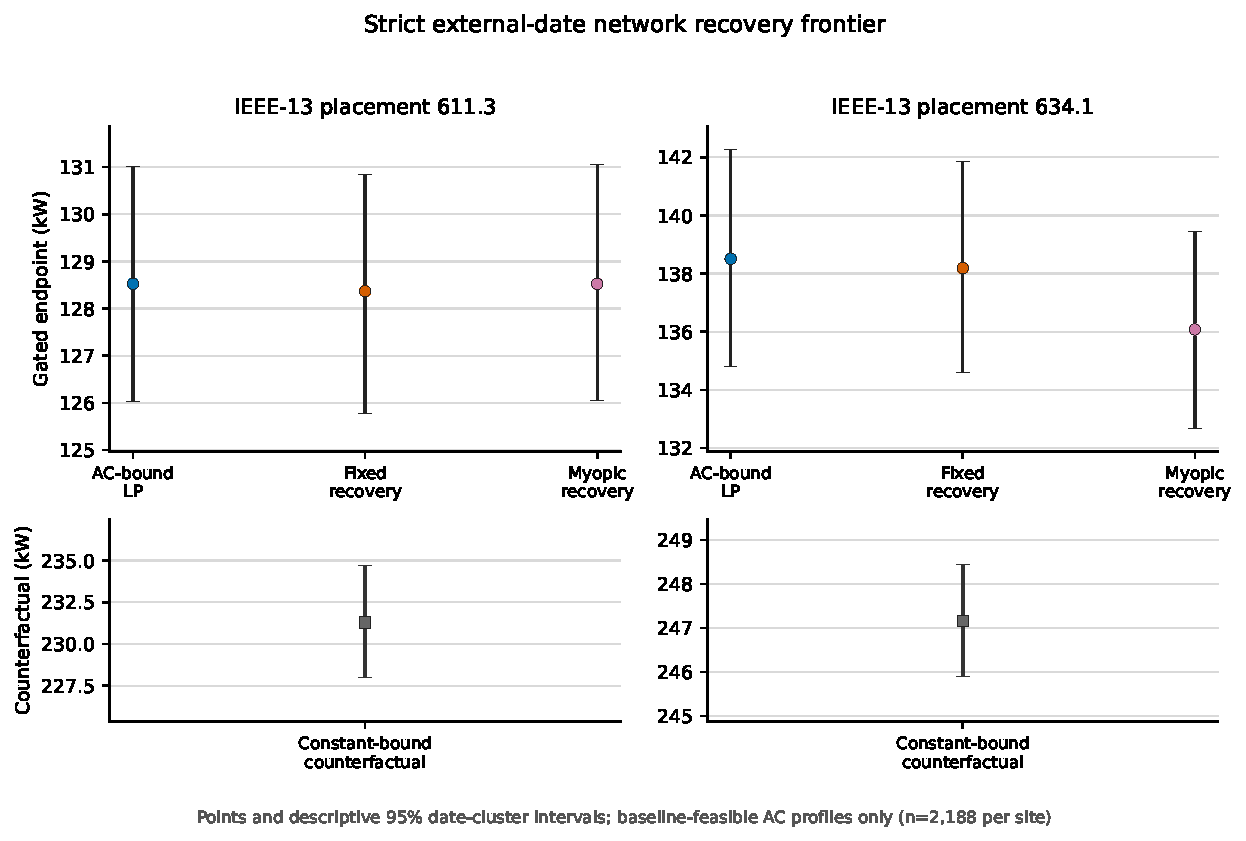
\includegraphics[width=0.99\linewidth]{fig1_external_frontier}
\caption{Mean feasible service power and descriptive 95\% date-cluster intervals over 2,188 baseline-AC-feasible units per placement. The constant-bound counterfactual is separated into its own lower panel because its magnitude would compress the three policy estimates; its schedules fail AC replay and are not deliverable offers.}
\label{fig:frontier}
\end{figure}

\subsection{Cross-source robustness}
The OPSD test block provides a source-level robustness check after the Ausgrid protocol was frozen. Table~\ref{tab:opsd} and Figure~\ref{fig:opsd} report 132 held-out dates for one household profile at each placement; all 264 zero-power gates passed. The AC-bound scalar LP endpoint is 114.551~kW at 611.3 and 145.816~kW at 634.1, with 100\% AC replay success for the network, fixed-recovery, and myopic schedules. The constant-bound counterfactual reaches 198.372 and 219.840~kW but has zero replay success. The resulting AC-bound-to-constant-bound ratios are 57.7\% and 66.3\%, which preserve the direction of the Ausgrid result while changing the source and the date range. The bootstrap intervals in Table~\ref{tab:opsd} are descriptive date-cluster intervals; because the OPSD check uses one household profile, it does not quantify customer-group uncertainty.

\begin{table}[t]
\centering
\caption{OPSD held-out cross-source robustness check on the same IEEE-13 feeder. Values are kW; the estimate and descriptive 95\% date-cluster interval are shown in separate columns, and the final row for each placement gives the network-to-constant-bound ratio. All 132 dates pass the zero-power gate.}
\label{tab:opsd}
\small
\begin{tabular}{llrr}
\toprule
Placement & Policy & Estimate (kW) & 95\% CI (kW)\\
\midrule
611.3 & AC-bound scalar LP & 114.551 & 111.813--117.165\\
611.3 & Fixed recovery & 114.486 & 111.719--117.178\\
611.3 & Myopic recovery & 114.551 & 111.803--117.175\\
611.3 & Constant-bound & 198.372 & 191.458--205.355\\
611.3 & $\rho_{\mathrm{CB}}$ & \multicolumn{2}{l}{0.577}\\
634.1 & AC-bound scalar LP & 145.816 & 141.993--149.377\\
634.1 & Fixed recovery & 145.816 & 142.020--149.377\\
634.1 & Myopic recovery & 145.816 & 141.948--149.307\\
634.1 & Constant-bound & 219.840 & 214.915--224.801\\
634.1 & $\rho_{\mathrm{CB}}$ & \multicolumn{2}{l}{0.663}\\
\bottomrule
\end{tabular}
\end{table}

\begin{figure}[t]
\centering
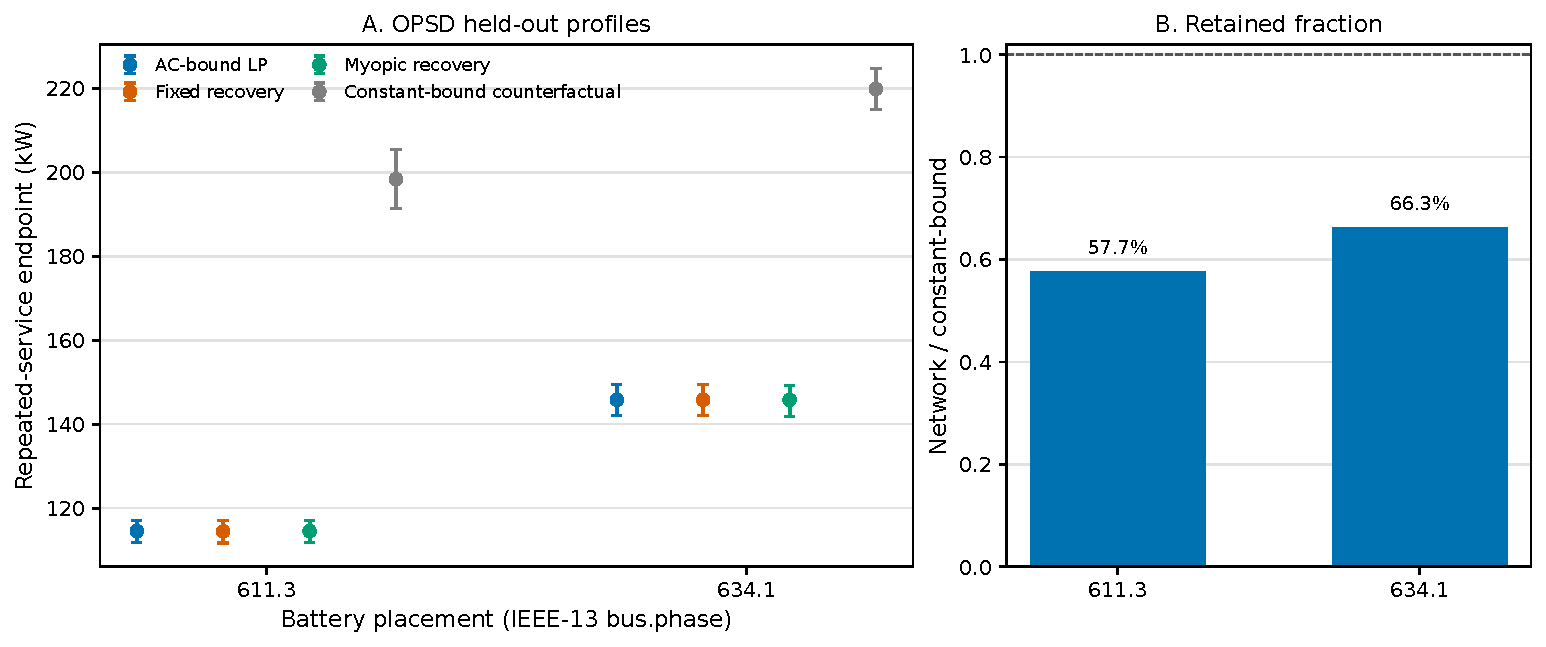
\includegraphics[width=0.99\linewidth]{fig2_opsd_cross_source_frontier}
\caption{OPSD held-out cross-source robustness check on the same IEEE-13 feeder. Panel A shows date-cluster service endpoints and descriptive intervals; panel B shows the network-to-constant-bound ratio. The check supports source robustness and does not establish cross-feeder transferability.}
\label{fig:opsd}
\end{figure}

\subsection{Capacity and contract-information horizon}
The capacity sweep in Figure~\ref{fig:capacity} shows two regimes under the frozen audited scalar bounds. At 634.1, the date-cluster AC-bound scalar-LP endpoint is 71.083~kW at 250~kWh, 127.009~kW at 500~kWh, and 138.511~kW at 1,000 and 2,000~kWh. The binding audit confirms the interpretation: the 250-kWh case is frequently below the service-window export envelope, whereas the larger cases reach that envelope for every baseline-gated unit. At 611.3, the corresponding values are 71.238, 124.559, and 128.526~kW at 250, 500, and 1,000~kWh; the 2,000-kWh value remains 128.526~kW.

The finite-information results in Table~\ref{tab:sensitivity} and Figure~\ref{fig:horizon} show the largest conditional recovery-rule sensitivity at 634.1 in this frozen-bound sensitivity. With $E=2000$~kWh, H4, H8, H12, and H24 achieve 45.044, 79.483, 108.389, and 136.078~kW, respectively, against 138.511~kW for the full-horizon audited endpoint. At 611.3, H8 already reaches 128.472~kW and H24 matches the full-horizon endpoint to the displayed precision. The pattern remains visible at intermediate capacities, but its interpretation is specific to the declared recovery rule and offline endpoint selection. After deterministic exact-terminal handling was applied, the greedy myopic rollout remained planner-feasible for all 2,188 baseline-gated units at 250~kWh at both placements; it is therefore retained as a recovery-rule comparator rather than interpreted as an online information effect. At this 2-MWh energy level, the initial SOC can support both calls at the reported network frontiers; the factorial mechanism audit shows that H4--H12 jointly reflect delayed service-start and terminal-target visibility, while the H24 residual gap is entirely due to the terminal-target rule. Exposing the terminal target at every recovery decision restores 138.511~kW even when service starts remain finite-horizon, whereas exposing all service starts while retaining finite terminal visibility gives 136.078~kW. These values are offline policy sensitivities indexed by a joint contract-information horizon, not communication-performance measurements.

The exact certificate in Eq.~\eqref{eq:capacity_certificate} was then audited against the existing HiGHS dispatch on all 4,376 baseline-gated units at the two primary placements. It identified a feasible capacity interval for every unit; the minimum capacity ranged from 165.022 to 711.349~kWh (median 465.735~kWh). Every active lower witness was a reachability cut over the first service window $[0,12)$, so the present sample's minimum-capacity distribution is primarily an initial-SOC bandwidth diagnostic; the general certificate also retains arbitrary intermediate-window cuts, which are covered by the synthetic regression tests. The LP was probed just below and above each certified lower boundary and at 2,000~kWh: all 13,128 of 13,128 feasibility labels matched. This is an exact audit of the scalar dispatch layer under frozen AC bounds; it does not replace the separate nonlinear replay or claim a physical capacity guarantee beyond the tested feeder model.

\begin{table}[t]
\centering
\caption{Date-cluster service-power sensitivity at placement 634.1. Values are kW; the finite-information recovery policies jointly restrict service-start and terminal-target visibility according to the stated horizon.}
\label{tab:sensitivity}
\resizebox{\linewidth}{!}{\begin{tabular}{lrrrrrr}
\toprule
$E$ (kWh) & AC-bound scalar LP & H4 & H8 & H12 & H24 & Myopic\\
\midrule
250  & 71.083 & 70.808 & 71.083 & 71.083 & 71.083 & 71.083\\
500  & 127.009 & 45.044 & 122.046 & 126.972 & 127.009 & 127.009\\
1000 & 138.511 & 45.044 & 79.483 & 108.389 & 138.067 & 138.067\\
2000 & 138.511 & 45.044 & 79.483 & 108.389 & 136.078 & 136.078\\
\bottomrule
\end{tabular}}
\end{table}

\begin{figure}[t]
\centering
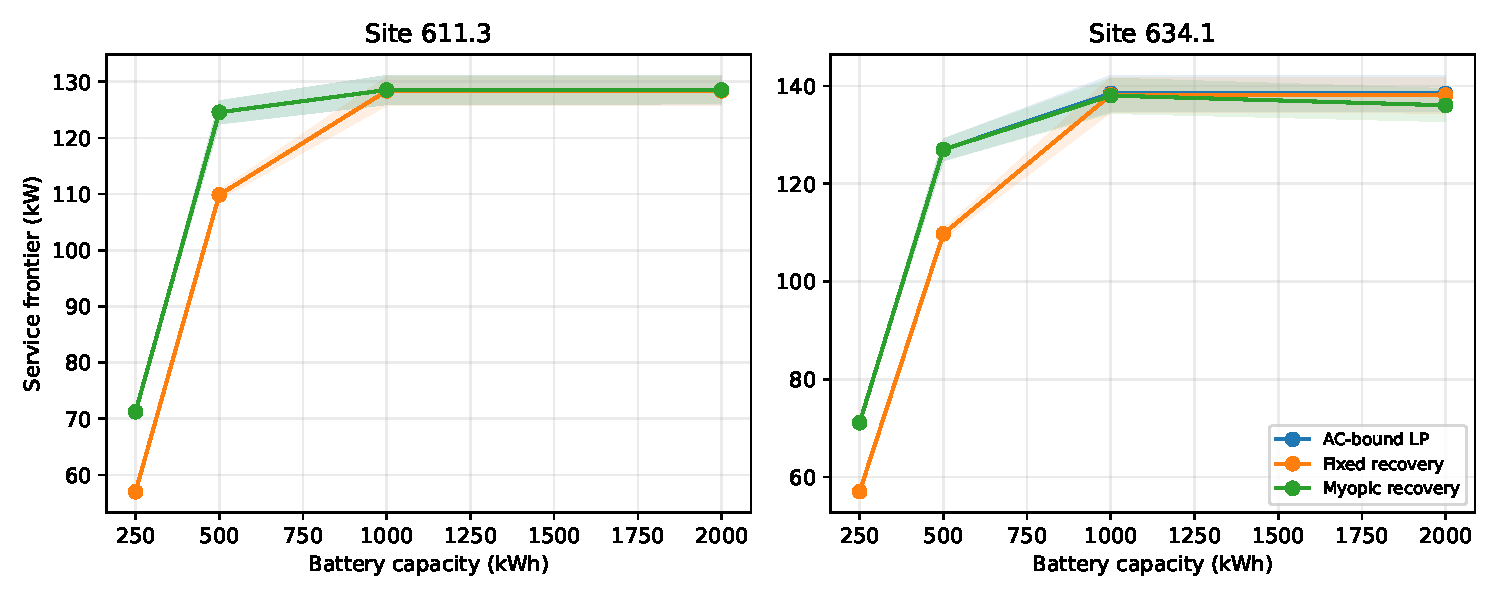
\includegraphics[width=0.99\linewidth]{capacity_frontier}
\caption{Capacity sensitivity under the audited scalar AC bounds. The frontier saturates near the network limit after 500--1000~kWh, while the fixed and myopic recovery responses differ between the two selected placements.}
\label{fig:capacity}
\end{figure}

\begin{figure}[t]
\centering
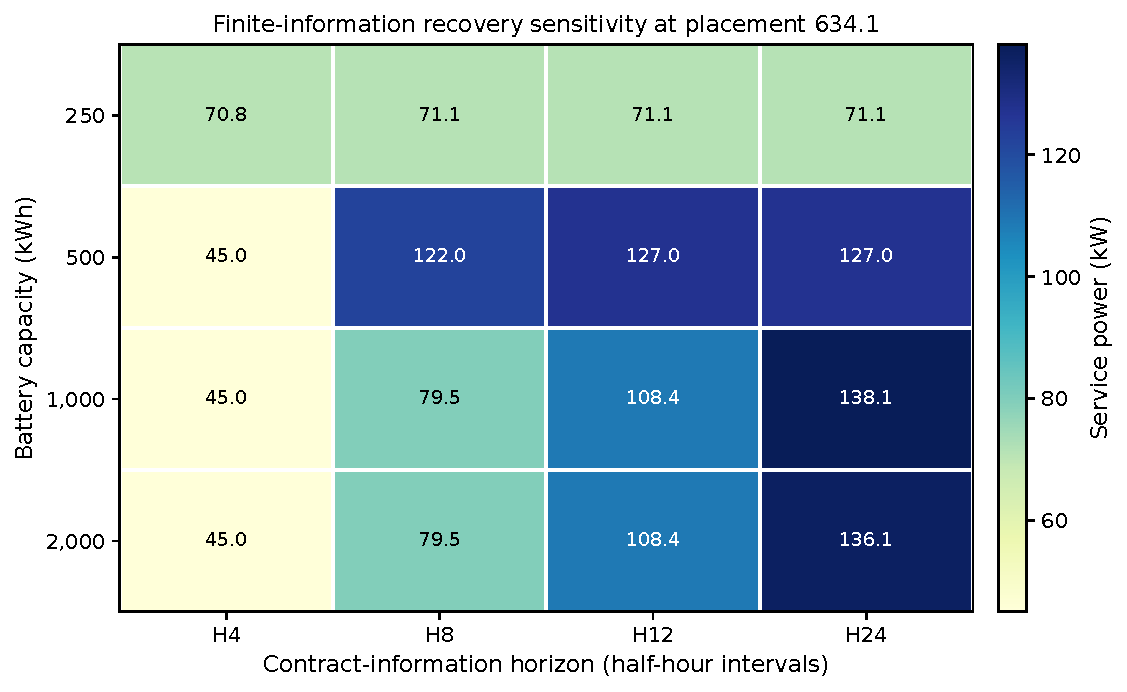
\includegraphics[width=0.82\linewidth]{causal_horizon_heatmap}
\caption{Finite-information recovery-policy sensitivity at placement 634.1 under frozen audited scalar AC bounds. Each cell is the date-cluster mean service power for a policy whose visibility of later service starts and the terminal SOC target follows the stated H horizon; endpoint selection is offline using the realized day.}
\label{fig:horizon}
\end{figure}


\subsection{Three-call chronological stress}
The complete three-call grid contains 70,016 baseline-gated rows with the terminal target always visible and the full service calendar declared. The earliest-charge implementation matched the scalar LP in every row, confirming that the relevant comparison is between exact cumulative chronology and its aggregate relaxation rather than between two optimizers. Figure~\ref{fig:threecall} summarizes the four second-call gaps and four capacities at both primary placements.

The only material contraction is at placement 634.1 with \(E=500\)~kWh and \(s=24\), where the second call starts after a 6~h gap from the first call. The exact endpoint is 122.614~kW, whereas the aggregate relaxation is 126.889~kW, giving \(\kappa_{\mathrm{chron}}=4.288\)~kW (date-cluster 95\% CI 3.784--4.834~kW). The contraction is positive for 1,141 of 2,188 units (52.148\%). The certificate identifies 1,127 witnesses crossing the intermediate interval \([24,36)\) and 14 witnesses extending through the terminal tail \([24,48)\). The shorter gaps and all capacities at this placement have no material residual after the aggregate cuts; the 611.3 site has only four positive rows at \(E=500\)~kWh and \(s=24\), with a non-material mean residual of \(0.018\)~kW. This localization supports a chronology mechanism tied to the recovery window between calls 2 and 3, rather than a generic capacity or terminal-information effect.

The selected \(E=500\)~kWh, \(s=24\) cell was replayed as a nonlinear OpenDSS snapshot audit for all 4,376 baseline-gated units. Joint planning and replay succeeded for 4,375 units (99.977\%): all 2,188 units at 611.3 and 2,187 at 634.1. The sole failure was a transformer-loading readback of 1.000001 at 634.1, just above the declared \(10^{-6}\) loading tolerance; it is retained as a tolerance edge and does not convert the scalar grid into a field-delivery guarantee.


In a separate stratified 200-unit diagnostic (10 retained dates, 10 groups, and both placements), every scalar endpoint also passed all 48 nonlinear snapshots, so the checked scalar-versus-replay endpoint gap was 0.000~kW in this sample. This is evidence about the sampled endpoints only; it does not prove that the product of independent interval bounds equals the joint nonlinear AC feasible set.

The same audit makes the model-dependence visible. Clipping the frozen scalar charge/export bounds by symmetric device caps gives mean endpoints of 79.925 and 79.579~kW at an 80-kW cap, 126.760 and 130.131~kW at 150~kW, and 128.530 and 138.507~kW at 200~kW, at 611.3 and 634.1 respectively; these are dispatch diagnostics without a nonlinear inverter model. A fresh six-date, two-group AC snapshot sample under alternative load/PV embeddings spans 74.010--183.294~kW across the tested variants (load gain, PV rating, and PV location). The placement and endpoint claims therefore remain conditional on the declared synthetic embedding.

The numerical protocol was also perturbed on a 40-unit sample. Replacing the 0.01-kW command readback floor by zero changed no endpoint; replacing the declared $10^{-6}$ voltage/loading tolerance by zero changed no endpoint at the 20-kW grid, while $10^{-5}$ increased the mean by 0.168~kW and the maximum by 0.313~kW. Using 10- and 40-kW coarse-grid steps changed endpoints by at most 0.039 and 0.078~kW, respectively, at the declared tolerance (0.156~kW at zero tolerance). These are sample diagnostics rather than full-population error bounds, and they support treating sub-0.1-kW differences as unresolved by the checked-prefix protocol.

\begin{figure}[H]
\centering
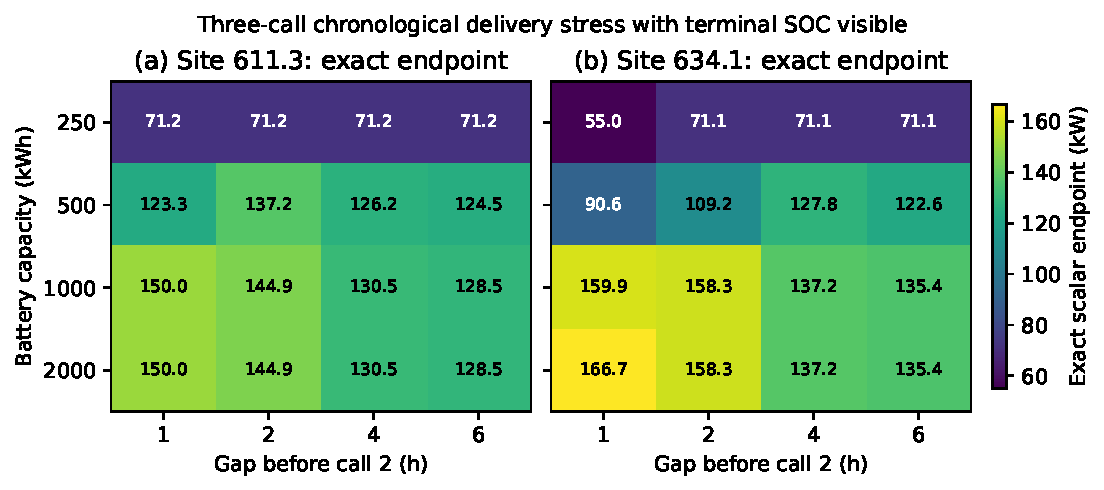
\includegraphics[width=0.99\linewidth]{three_call_chronology_grid}
\caption{Predeclared three-call chronology stress under an always-visible terminal target. The two panels show exact scalar-LP endpoints across capacity and second-call gap at the two primary placements. The associated aggregate-relaxation contraction is reported in the Results text; its only material residual is the $E=500$~kWh, $s=24$ cell at 634.1 ($4.288$~kW).}
\label{fig:threecall}
\end{figure}

\subsection{Headroom-margin stress}
Figure~\ref{fig:headroom} shows that the network-audited limit also decreases smoothly when an operator withholds part of the audited interval envelope. At 634.1, multiplying every charge and export bound by 0.95, 0.90, and 0.80 reduces the AC-bound scalar LP estimate from 138.511 to 131.585, 124.659, and 110.808~kW, respectively. At 611.3, the corresponding values are 128.526, 122.099, 115.673, and 102.821~kW. The AC-bound scalar-LP--myopic gap at 634.1 contracts from 2.433~kW at zero margin to 1.946~kW at a 20\% margin, showing that the information effect is partly masked when the feeder envelope is made uniformly conservative. This stress test is useful for screening but remains a reduced scalar-bound sensitivity rather than a forecast-error or uncertainty guarantee.

% Keep the headroom stress figure with its Results subsection; the explicit H
% placement prevents this float from crossing the Results--Discussion boundary.
\begin{figure}[H]
\centering
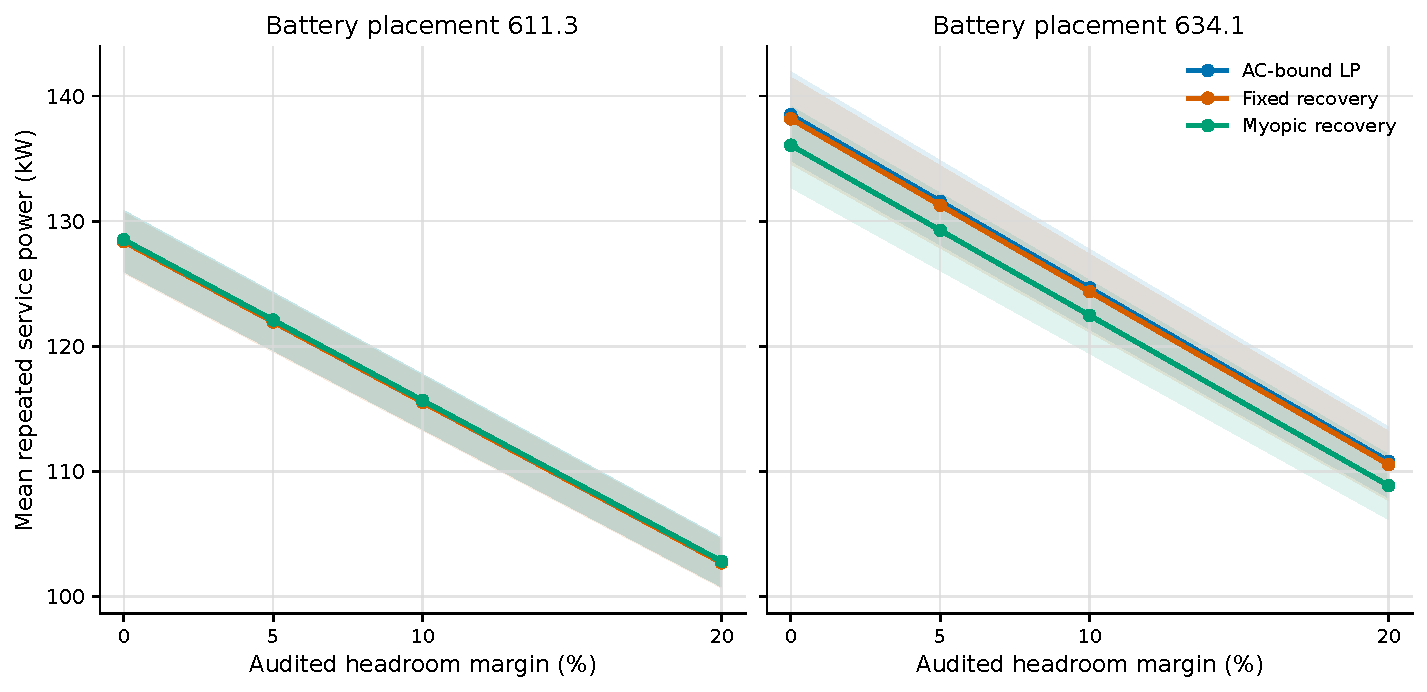
\includegraphics[width=0.99\linewidth]{headroom_margin_frontier}
\caption{Deterministic headroom-margin stress of the network-audited repeated-flexibility screening endpoint. Shaded bands are descriptive date-cluster intervals; multiplying all audited charge/export bounds by $(1-m)$ is a scalar-bound stress, not a probabilistic forecast model.}
\label{fig:headroom}
\end{figure}

\subsection{Empirical screening threshold}
The retained-sample screening curves are shown in Figure~\ref{fig:safeoffer}. At a target empirical coverage of 95\%, the AC-bound scalar LP descriptive lower-tail empirical screening threshold over retained baseline-AC-feasible units is 89.297~kW at 611.3 and 83.203~kW at 634.1. The frontier coverages are 0.9502 at both placements, and the mean shortfall energies are 1.378 and 2.246~kWh per retained unit. The new fixed-threshold AC replay gives the same 0.9502 replay coverage at both placements: 2,079 of 2,188 baseline-gated units have a planner-feasible common-power schedule and every one of those schedules passes the nonlinear replay. The constant-bound counterfactual reports 188.180 and 220.730~kW at the same target, but its checked-prefix scalar service-window export bounds are below those thresholds for every retained unit; this is a certificate within the audited reduced model that the counterfactual values are not deliverable under those bounds. The endpoint therefore exposes the optimism created by removing temporal variation from the audited envelope without assigning an arbitrary price or calling the sample quantile a guarantee.

\begin{figure}[H]
\centering
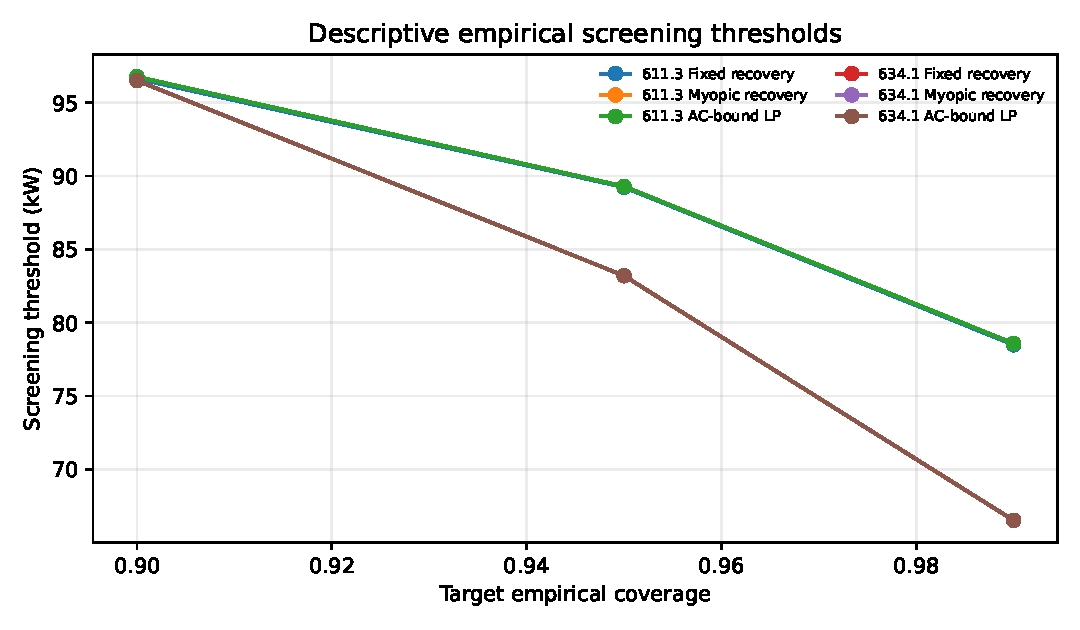
\includegraphics[width=0.99\linewidth]{safe_offer_frontier}
\caption{Descriptive empirical lower-tail screening thresholds over baseline-AC-feasible units. The curves summarize retained-sample coverage; the 95\% AC-bound scalar-LP thresholds are separately evaluated as common-power schedules in the fixed-threshold AC replay audit. Neither statistic is a probabilistic guarantee for future events.}
\label{fig:safeoffer}
\end{figure}

\subsection{AC replay and failure audit}
Figure~\ref{fig:failure} summarizes the conditional AC replay outcomes. The full-horizon and fixed-recovery schedules replayed successfully on all 2,188 baseline-feasible units at both placements. The myopic schedule also replayed successfully at 611.3 and on 2,187 of 2,188 units at 634.1; the single failed replay occurred at interval 34 for group 6 on 14 January 2013, when transformer \texttt{xfm1} exceeded the declared loading tolerance by a small numerical margin. No voltage failure was recorded for this unit. The constant-bound counterfactual schedule failed on all 2,188 baseline-feasible units at both placements. Its service power is therefore a diagnostic of temporal-network optimism, not a feasible contract.

\begin{figure}[H]
\centering
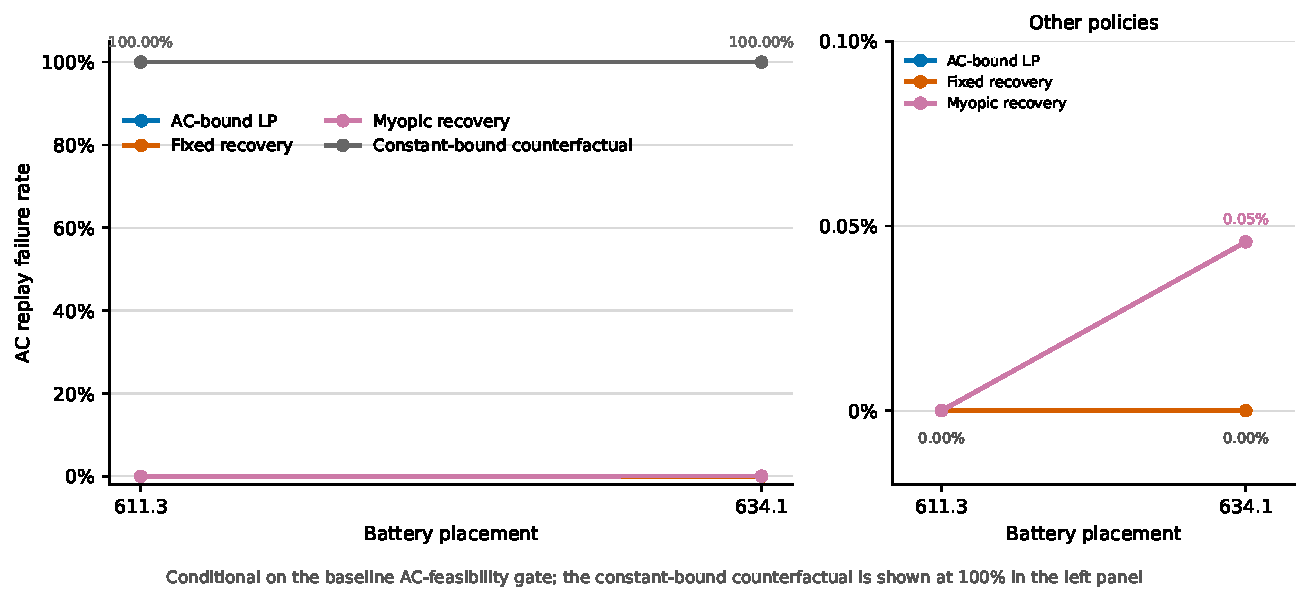
\includegraphics[width=0.99\linewidth]{fig3_failure_rates}
\caption{Conditional AC replay failure rates. The left panel retains the 100\% constant-bound counterfactual failure rate; the right panel resolves the much smaller rates of the other policies.}
\label{fig:failure}
\end{figure}

\subsection{Recovery trajectory and headroom mechanism}
The representative trace in Figure~\ref{fig:trace} shows that service calls and recovery windows occur at different AC charge limits. The full-horizon policy moves charging within the allowed recovery windows to satisfy the second call and the terminal SOC, whereas fixed recovery follows the same ratio regardless of the time-varying limit. At 634.1, the observed LP--myopic difference is positively associated with the recovery-window charge-headroom range divided by its mean (Spearman $\rho=0.440$; Pearson $r=0.508$ over 2,188 paired units). At 611.3, the LP--myopic difference is identically zero, so its correlation is undefined. Figure~\ref{fig:mechanism} visualizes this association. These correlations are descriptive and do not establish a causal effect of placement.

\begin{figure}[t]
\centering
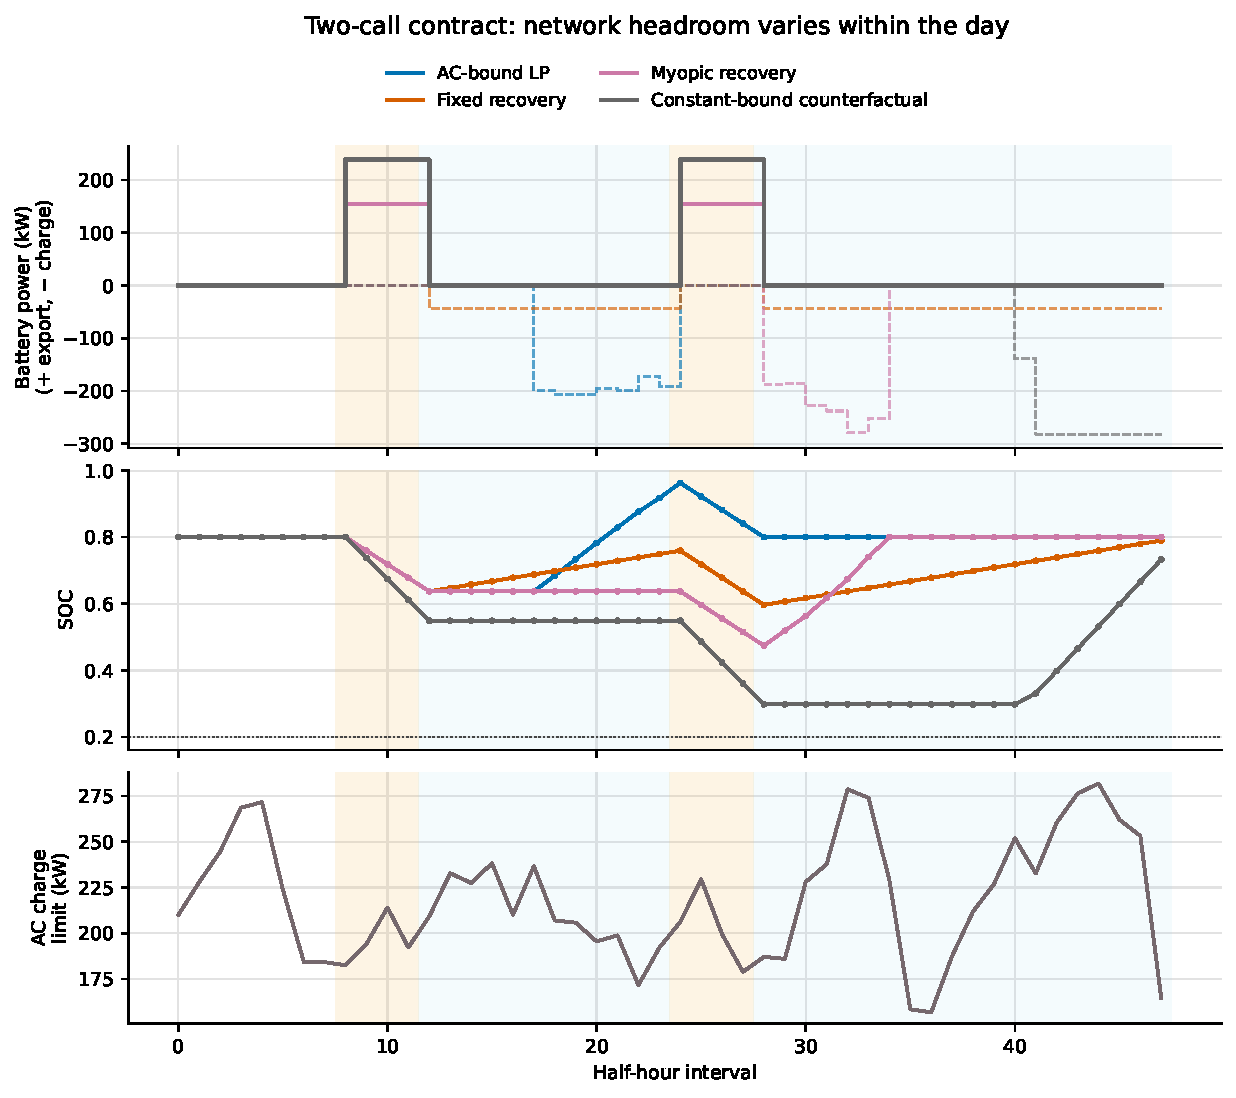
\includegraphics[width=0.99\linewidth]{fig2_recovery_trace}
\caption{Representative 48-interval trace. Gold shading marks the two service windows and blue shading marks the recovery windows. Solid curves show export; dashed curves show charging as negative battery power.}
\label{fig:trace}
\end{figure}

\begin{figure}[t]
\centering
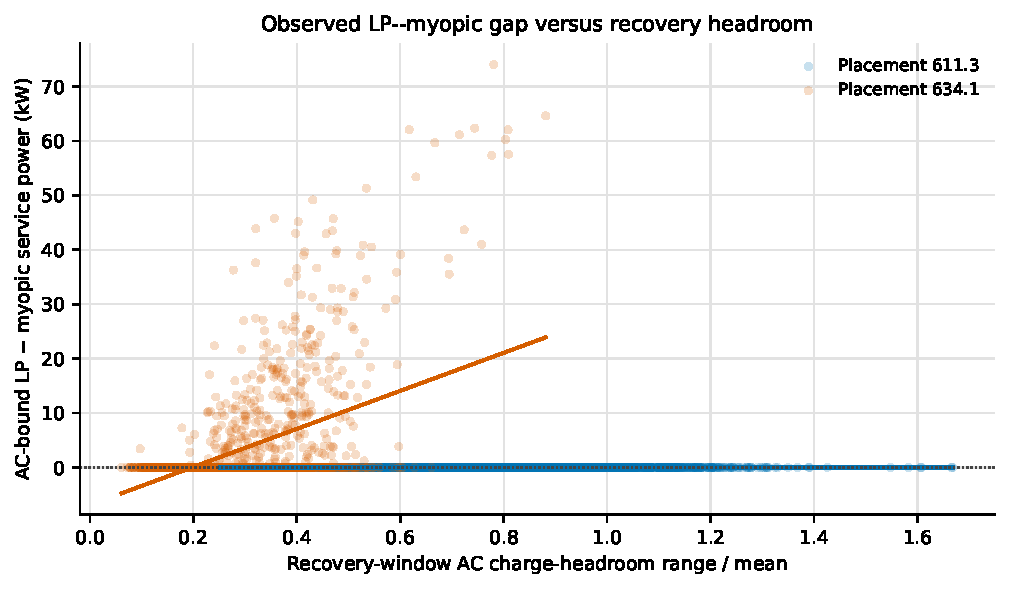
\includegraphics[width=0.82\linewidth]{fig4_headroom_mechanism}
\caption{Observed LP--myopic service-power difference against the recovery-window AC charge-headroom range divided by its mean. Lines are descriptive fits; the plot is not a causal test.}
\label{fig:mechanism}
\end{figure}

\subsection{Placement-conditioned extension}
The predeclared seven-site extension in Figure~\ref{fig:location} converts the two-placement comparison into a within-feeder location screen. The zero-power gate passed 2,188 of 2,190 units at every site. Conditional date-cluster AC-bound scalar LP endpoints ranged from 112.020~kW at 646.3 to 148.059~kW at 675.1, where the battery is co-located with the fixed-P PV surrogate; the primary placements reproduced 128.526~kW at 611.3 and 138.511~kW at 634.1. The AC-bound scalar-LP--myopic difference was largest at 675.1 (6.232~kW, 95\% CI 4.567--7.990~kW) and remained 2.433~kW (1.690--3.261~kW) at 634.1, while it was zero to the displayed precision at 611.3, 645.3, 646.3, and 684.3. The 2-MWh binding audit found exact equality between the AC-bound scalar-LP endpoint and the minimum service-window export bound for all 2,188 baseline-feasible units at each site. Nonlinear replay was complete for the network policy at 611.3, 634.1, and 675.1; it passed for 2,184/2,188 units at 652.1 and 2,185/2,188 units at 645.3, 646.3, and 684.3. The few failures were voltage readback values 1~\texttimes~10$^{-6}$ pu above the stated tolerance. This map supports a placement-conditioned location--service screen, while its single-feeder scope remains explicit.

\begin{figure}[t]
\centering
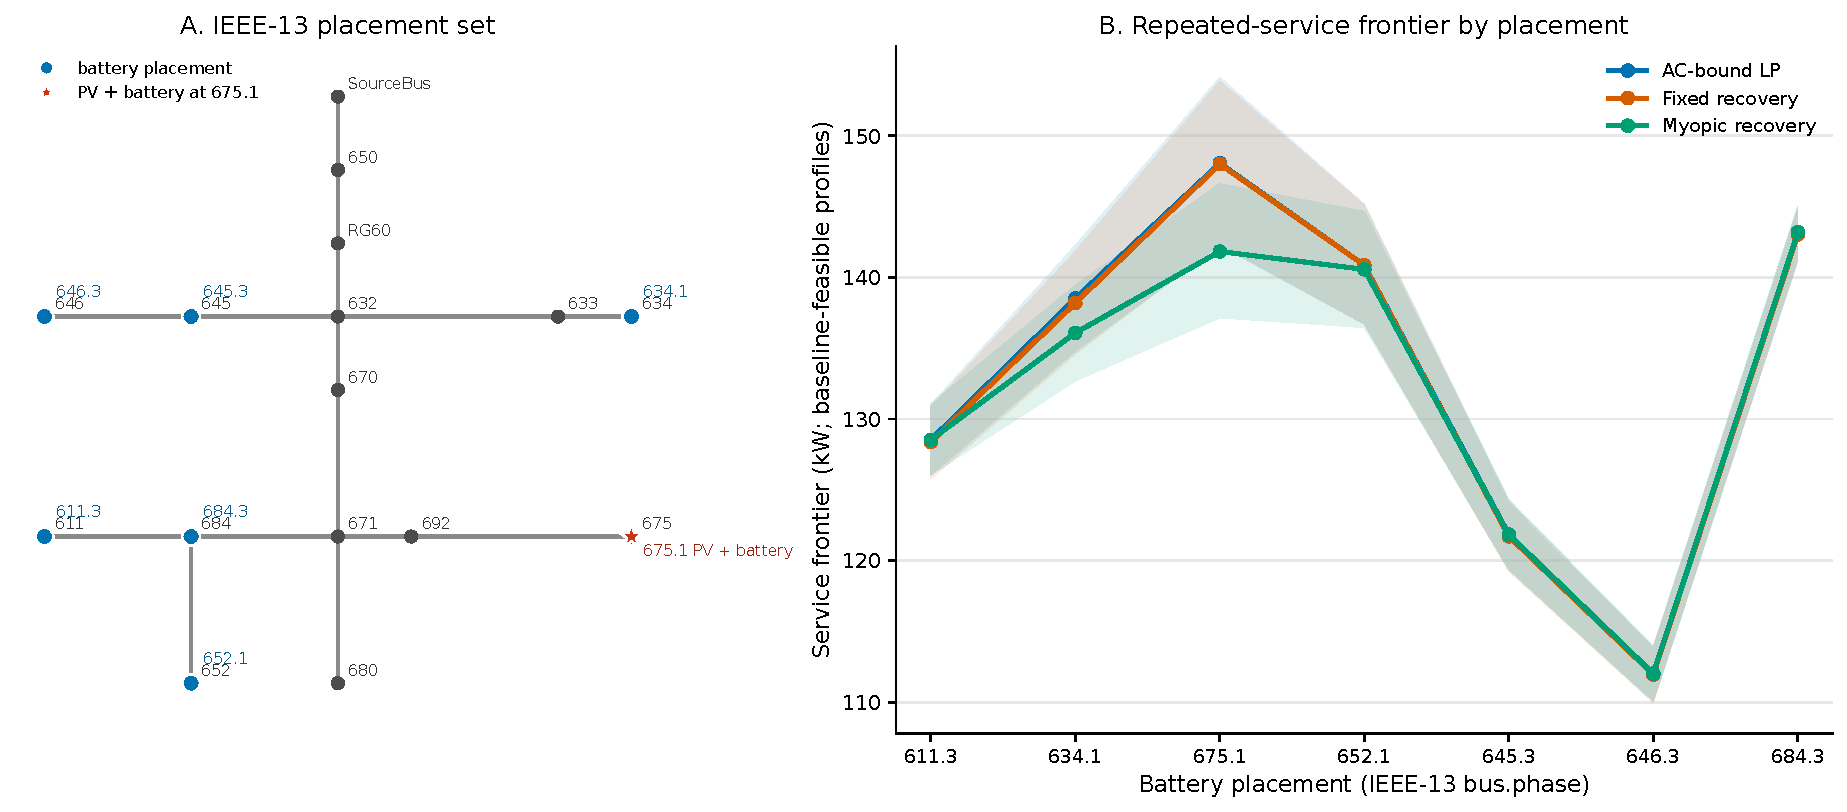
\includegraphics[width=0.99\linewidth]{location_frontier}
\caption{Within-feeder placement sensitivity of the repeated-service frontier. Panel A shows the IEEE-13 topology and the seven predeclared battery bus-phase placements, with the PV-coincident site 675.1 marked separately; panel B shows date-cluster means and descriptive 95\% intervals over 2,188 baseline-AC-feasible units per site. The map is a placement-conditioned screen, not an all-bus placement law.}
\label{fig:location}
\end{figure}

\subsection{Temporal evaluation of a common cross-placement offer}
The common-offer experiment in Figure~\ref{fig:commonoffer} selects one power from the pooled 2012 calibration block and evaluates it without site-specific retuning in the retained 2013 block. The lower 5th percentile of 7,203 baseline-gated AC-bound scalar LP endpoints is 79.453~kW; using linear interpolation, 6,843 units (95.002\%) are at or above this calibration endpoint. The fixed-power LP and nonlinear replay are then applied to 8,113 baseline-gated 2013 units across the seven sites. The joint planner-plus-replay success is 99.150\% (descriptive date-cluster 95\% interval 98.510--99.643\%), with 8,044 of 8,045 planner-feasible schedules passing nonlinear replay at the declared $10^{-6}$ pu/loading readback tolerance. Including the seven zero-power gate failures as automatic failures gives 8,044/8,120 physical evaluation units, or 99.064\% unconditional screening success. By retained evaluation block, the unconditional joint rates are 1,701/1,750 = 97.200\% for 2013-01-01--2013-01-25 (including the seven gate failures) and 6,343/6,370 = 99.576\% for 2013-04-01--2013-06-30; these are block summaries rather than season-level population estimates. The sole strict replay failure is retained at site 652.1 on 29 April 2013 for group 6, where a marginal voltage readback exceeded the tolerance. Table~\ref{tab:commonoffer} reports the site denominators, planner coverage, conditional replay coverage, and date-cluster intervals; joint success ranges from 98.188\% at the PV-coincident site 675.1 to 100.000\% at 684.3. The mean scalar-frontier shortfall diagnostic is 0.216~kWh per unit (descriptive date-cluster 95\% interval 0.069--0.398~kWh), computed as the positive local AC-bound scalar LP endpoint gap over four service hours; it is not measured unmet energy from the AC replay. The offer is therefore a useful retained-sample screening result with a temporal calibration/evaluation split, while its interpretation remains conditional on the frozen feeder and profile embedding.

\begin{table}[t]
\centering
\caption{Site-level evaluation of the fixed retained-sample common screening offer. Rates are percentages over the 1,159 baseline-gated units at each site. The conditional replay rate is computed only among planner-feasible schedules; intervals are descriptive 95\% date-cluster intervals for the joint planner-plus-replay rate. The pooled unconditional screen is 8,044/8,120 because seven zero-power gate failures are counted as automatic failures.}
\label{tab:commonoffer}
\small
\begin{tabular}{lrrrr}
\toprule
Site & $n$ & Planner & Replay $\mid$ planner & Joint (95\% CI)\\
\midrule
611.3 & 1,159 & 99.83 & 100.00 & 99.83 (99.57--100.00)\\
634.1 & 1,159 & 98.62 & 100.00 & 98.62 (97.41--99.57)\\
645.3 & 1,159 & 99.57 & 100.00 & 99.57 (99.14--99.91)\\
646.3 & 1,159 & 99.40 & 100.00 & 99.40 (98.97--99.74)\\
652.1 & 1,159 & 98.53 & 99.91 & 98.45 (97.24--99.40)\\
675.1 & 1,159 & 98.19 & 100.00 & 98.19 (96.81--99.22)\\
684.3 & 1,159 & 100.00 & 100.00 & 100.00 (100.00--100.00)\\
\bottomrule
\end{tabular}
\end{table}

\begin{figure}[t]
\centering
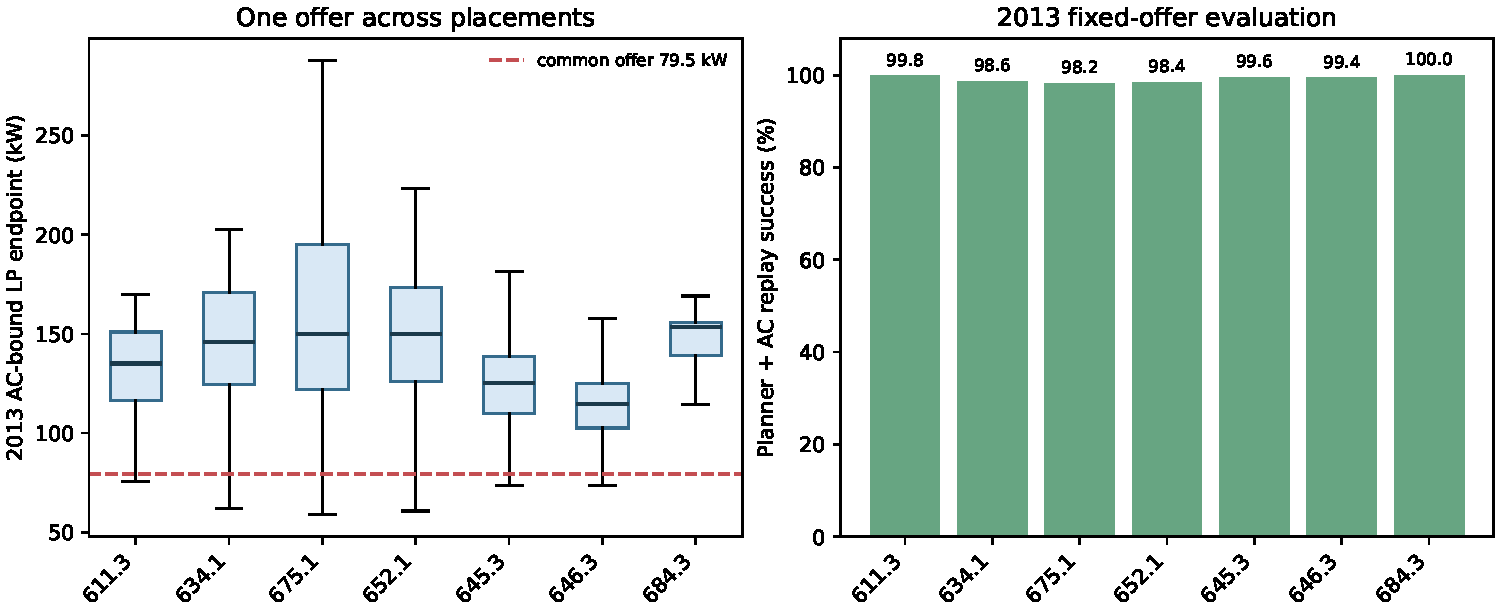
\includegraphics[width=0.99\linewidth]{common_offer_temporal_evaluation}
\caption{Cross-placement temporal evaluation of one fixed common offer. The offer is calibrated from the pooled 2012 AC-bound scalar LP lower 5th percentile and evaluated without site-specific retuning on the retained 2013 block. Boxplots show local AC-bound scalar LP endpoints; bars show joint fixed-power planning and nonlinear AC replay success. The evaluation is a descriptive screening result, not a future delivery guarantee.}
\label{fig:commonoffer}
\end{figure}

\subsection{Capacity falsification of the pooled lower-tail offer}
To test whether the pooled common offer was being set by battery energy rather than the feeder envelope, we repeated the calibration/evaluation protocol at $E=500$~kWh with the same SOC fractions, exact terminal target, seven sites, and strict nonlinear replay. The capacity-aware AC-bound scalar LP and the service-window export-floor comparator both selected 79.453~kW from the 7,203-unit 2012 calibration block. On the 8,113-unit 2013 evaluation block, both offers had 8,045 planner-feasible schedules and 8,043 joint planner--replay successes (99.137\% unit-weighted; date-cluster estimate 99.138\%, 95\% CI 98.522--99.618\%). The 68 planner failures were all audited export-limit failures; the two replay failures were voltage-readback failures at 645.3 on 21 January 2013 (group 1) and 652.1 on 29 April 2013 (group 6). No failure was classified as SOC or terminal infeasibility. The row-level $E=500$ endpoint distribution is lower than the service-window floor for 2,230 of 7,203 calibration units, but the pooled lower 5\% tail is unchanged. This falsification therefore bounds the interpretation of the common offer: its observed lower-tail limit is export-floor dominated, while capacity and SOC recovery remain modeled sensitivity dimensions rather than demonstrated bottlenecks of that offer.

% Flush Results floats before Discussion so figures remain in the Results section.
\clearpage
\section{Discussion}
The three-call audit supplies the manuscript's central chronology result. With the terminal target always visible and the service calendar fully declared, the scalar greedy implementation and LP coincide across all 70,016 rows, while the aggregate relaxation fails only when the second call at 634.1 is separated from the first by 6~h at \(E=500\)~kWh. The exact endpoint is 122.614~kW versus 126.889~kW for the aggregate bound, a 4.288-kW contraction with a date-cluster interval of 3.784--4.834~kW and positive rows in 52.148\% of the population. The active cumulative witnesses cross \([24,36)\), and the selected cell survives nonlinear replay for 4,375/4,376 baseline-gated units. This is evidence of an intermediate recovery-window constraint within the tested scalar contract, not a communication-performance claim or a universal chronology law.

The two-call 2-MWh endpoint remains service-window-export-bound limited under the tested protocol: the binding audit finds equality with the minimum audited export bound for every baseline-gated unit at all seven placement sites. The independent OPSD profile-source check preserves the temporal-envelope comparison, with AC-bound-to-constant-bound ratios of 57.7--66.3\% across its two placements versus 55.6--56.0\% for Ausgrid. Because both checks use the same IEEE-13 feeder and synthetic profile embedding, this is evidence of source robustness for the envelope diagnostic rather than evidence that the endpoint transfers across feeders. The seven-site map shows that location changes the absolute service envelope and can change the size of the hindsight AC-bound scalar-LP--myopic gap, with the largest observed gap at the PV-coincident site 675.1. The \(E=500\) falsification shows that the pooled lower-tail common offer remains set by the service-window export floor even when row-level capacity-aware endpoints are lower for 2,230 of 7,203 calibration units; the associated planner failures remain export-limit failures. The older H4--H24 analysis is retained as a bounded joint service-calendar/terminal-target sensitivity; it is not used as evidence of marginal communication value.

For a screening workflow, the outputs should be read in that order: first reject a candidate operating point that fails the zero-power AC gate; next inspect the full-horizon endpoint and its replay record; then increase capacity until the frozen-bound frontier saturates; finally report the declared-calendar sensitivity and the descriptive lower-tail threshold with its non-guarantee label. This sequence turns the experiment into a capacity-and-contract screen for a DSO or aggregator, while leaving forecast, market, and field-control decisions to a later model.
The resulting DSO/aggregator decision chain is explicit but deliberately technical: (i) reject a site--date--group unit that fails the zero-power gate; (ii) use the AC-bound scalar-LP endpoint as a candidate bid limit only after checking its replay record; (iii) apply the declared recovery-calendar and terminal-SOC rules; and (iv) escalate a proposed activation or offer whenever the common threshold, replay audit, or baseline gate fails. The endpoint can therefore screen a bid limit or battery-capacity choice, but this study does not assign a market price, activation probability, penalty, or avoided-cost value. Any economic procurement decision requires those additional inputs.

For a concrete retained-sample screen, the seven-site temporal experiment selects one 79.453~kW offer from the pooled 2012 lower 5th percentile and evaluates it on the retained 2013 block. It is jointly planner- and replay-feasible for 8,044 of 8,113 baseline-gated units (99.150\%, descriptive date-cluster 95\% interval 98.510--99.643\%). Including seven zero-power gate failures gives 8,044/8,120 = 99.064\% unconditional screening success; this fixed offer is therefore a clearer cross-placement screen than the earlier site-specific thresholds. An operator can use it only as a descriptive pre-offer technical filter after the zero-power gate, while escalating any forecast, uncertainty, penalty, or market requirement to a model outside the present study.

The result is narrower than a chance-constrained procurement policy. The full-horizon policy sees the realized future and does not price flexibility, model forecast error, or optimize a market-clearing objective. The bootstrap intervals describe variation in the retained profile sample; they are not delivery guarantees for unobserved events. The 2012-to-2013 common-offer result is a temporal evaluation over retained non-contiguous blocks, not an untouched continuous-year holdout. The small placement-dependent effect also shows why a generic claim that AC-bound recovery always improves an offer would be unsupported by this experiment.

\section{Limitations}
The quantitative AC study uses one public IEEE 13-node feeder and seven predeclared single-phase placements; the OPSD experiment adds a profile-source robustness check on two of those placements, but no cross-feeder transfer claim is made. The three-call grid is a complete scalar-bound audit at two placements and four capacities, while nonlinear replay is limited to the predeclared \(E=500\)~kWh, \(s=24\) cell. The IEEE 123-node model is retained only as an adapter diagnostic because its operating-point data and ratings are not frozen for a transfer study. The battery is an active-power surrogate with fixed efficiencies and \(Q=0\); inverter apparent-power limits, reactive power, degradation, temperature, protection actions, ramping, and field telemetry are not represented. Snapshot AC bounds and replay establish model-based feasibility, not physical delivery. The public profiles are embedded by globally scaling all native feeder load phases and placing the fixed-P PV surrogate at 675.1, with controls held off; this synthetic stress embedding is not a calibrated customer-to-bus allocation. The binding and cumulative-window audits are exact for the tested scalar model, not proofs that the same witnesses persist in other capacities, feeders, or contracts. The \(E=500\) falsification specifically shows that changing capacity alone does not change the pooled lower-tail common offer or create SOC-classified planner failures under this feeder and offer rule. The capacity, finite-information, headroom-margin, and three-call sweeps reuse scalar AC bounds and do not rerun the nonlinear feeder for every cell; they are dispatch sensitivities under frozen audited scalar bounds. The quantile curves remain descriptive; the common-offer experiment adds a pooled 2012 calibration and retained 2013 evaluation with fresh fixed-power AC replay. Its reported 0.216-kWh value is a scalar-frontier shortfall diagnostic rather than AC-measured unmet energy, and the experiment still does not model forecast error, online adaptation, or a market guarantee. The finite-information policy uses perfect current bounds and hindsight endpoint selection, while the three-call chronology stress assumes the service calendar and terminal target are visible. Finally, the external dates are non-contiguous after a strict completeness mask, and the single replay edge at 634.1 shows why the result remains a screening benchmark rather than a delivery guarantee.

\section{Conclusions}
We developed a network-audited chronological delivery endpoint for repeated distribution-flexibility services. The decisive three-call audit used an always-visible terminal target and a complete 70,016-row gap-by-capacity grid; its greedy implementation matched the scalar LP in every row. At placement 634.1, \(E=500\)~kWh and a 6-h gap before the second call produced a 122.614-kW exact endpoint against a 126.889-kW aggregate relaxation, with a 4.288-kW contraction and 52.148\% positive rows. The selected cell passed nonlinear replay for 4,375/4,376 baseline-gated units. This identifies a localized intermediate recovery-window limit after aggregate service-floor and energy relaxations, within the tested scalar contract.

The two-call 2-MWh endpoint remains export-floor dominated: the full-horizon values are 128.526~kW at 611.3 and 138.511~kW at 634.1, while the seven-site map spans 112.020--148.059~kW. A single 79.453-kW offer calibrated on pooled 2012 endpoints was jointly planner- and replay-feasible for 8,044 of 8,113 retained 2013 units (99.150\%, descriptive date-cluster 95\% interval 98.510--99.643\%); including seven zero-power gate failures, the unconditional rate is 8,044/8,120 = 99.064\%. The \(E=500\) falsification assigned all 68 planner failures to export limits, and the OPSD check preserved the temporal-envelope comparison under a second profile source on the same feeder. These results support a reproducible DSO/aggregator screening workflow, conditional on the feeder, synthetic profile embedding, ideal active-power battery, scalar-bound assumptions, nonlinear replay cell, non-contiguous temporal blocks, and offline endpoint selection. Forecast-aware control, reactive-power inverter limits, additional feeders, and an economic objective remain necessary before a market recommendation can be made.

% All result floats were flushed before Discussion. Repeat the barrier here so
% no result figure can cross into the declarations or reference list after a
% later layout change.
\clearpage
\section*{CRediT authorship contribution statement}
\textbf{Siqiang Zhao:} Conceptualization, Methodology, Software, Validation, Formal analysis, Investigation, Data curation, Visualization, Writing -- original draft. \textbf{Fengxiang Zhang:} Supervision, Writing -- review \& editing. The author order and contribution statement were confirmed by both authors.

\section*{Funding}
No dedicated external funding was received for this work.

\section*{Declaration of competing interest}
The authors declare that they have no known competing financial interests or personal relationships that could have appeared to influence the work reported in this paper.

\section*{Acknowledgements}
No additional acknowledgements are requested.

\section*{Data and code availability}
The exact v5 source snapshot, result files, figure files, and SHA-256 manifests are supplied in the pre-submission bundle and frozen in the immutable GitHub tag \url{https://github.com/Zhaosiqiang/RecoveryFlex-AE/tree/v5.0.0}. The repository tag is the code and provenance identifier for this manuscript; a persistent DOI has not been assigned. No private participant-level data are claimed.

\section*{Declaration of generative AI and AI-assisted technologies in the writing process}
During preparation of this manuscript, the authors used OpenAI Codex/ChatGPT (platform-managed model, accessed in October 2026) for code organization, manuscript drafting, and internal consistency checks. No generative AI image tool was used to create or alter the data visualizations or graphical abstract; all figures were generated by deterministic scripts from the declared data and results. The authors reviewed and edited the assisted material and take full responsibility for the scientific content, data handling, figures, and final text. No AI tool is an author and no confidential or restricted data were provided to an AI tool.

{\small
\begin{thebibliography}{17}
\bibitem{Evans2022Recovery} M. P. Evans, S. H. Tindemans, D. Angeli, Flexibility framework with recovery guarantees for aggregated energy storage devices, IEEE Trans. Smart Grid 13 (2022) 3519--3531. doi:10.1109/TSG.2022.3173900.
\bibitem{Giraldo2023RiskEV} J. S. Giraldo, N. B. Arias, P. P. Vergara, M. Vlasiou, G. Hoogsteen, J. L. Hurink, Estimating risk-aware flexibility areas for electric vehicle charging pools via AC stochastic optimal power flow, J. Mod. Power Syst. Clean Energy 11 (2023) 1247--1256. doi:10.35833/MPCE.2022.000452.
\bibitem{Xiao2025SRC} J. Xiao, C. Li, G. He, Z. Lv, G. Sun, Y. Zhou, H. Liang, Flexible resource security regulating capability for distribution systems: Concept, method, and applications, Applied Energy 382 (2025) 125253. doi:10.1016/j.apenergy.2024.125253.
\bibitem{Lankeshwara2025DOE} G. Lankeshwara, R. Sharma, M. R. Alam, R. Yan, T. K. Saha, Development and validation of a dynamic operating envelopes-enabled demand response scheme in low-voltage distribution networks, Applied Energy 382 (2025) 125150. doi:10.1016/j.apenergy.2024.125150.
\bibitem{Cheng2026FOR} T. Cheng, J. Dai, D. Qiu, Z. Han, H. Sheng, H. Zhong, G. Strbac, Q. Xia, C. Kang, Coordinated optimal dispatch of storage-like resources based on dynamic feasible operation region aggregation, Applied Energy 424 (2026) 128444. doi:10.1016/j.apenergy.2026.128444.
\bibitem{Ji2019Flexibility} H. Ji, C. Wang, P. Li, G. Song, H. Yu, J. Wu, Quantified analysis method for operational flexibility of active distribution networks with high penetration of distributed generators, Applied Energy 239 (2019) 706--714. doi:10.1016/j.apenergy.2019.02.008.
\bibitem{Wanapinit2022FlexBidding} N. Wanapinit, J. Thomsen, A. Weidlich, Integrating flexibility provision into operation planning: A generic framework to assess potentials and bid prices of end-users, Energy 261 (2022) 125261. doi:10.1016/j.energy.2022.125261.
\bibitem{Wang2026Communication} S. Wang, Z. Wu, M. Zhou, Communication-dependent flexibility planning in digitalized distribution systems via dynamic storage reservation, Applied Energy 426 (2026) 128736. doi:10.1016/j.apenergy.2026.128736.
\bibitem{Klyapovskiy2019VoF} S. Klyapovskiy, S. You, A. Michiorri, G. Kariniotakis, H. W. Bindner, Incorporating flexibility options into distribution grid reinforcement planning: A techno-economic framework approach, Applied Energy 254 (2019) 113662. doi:10.1016/j.apenergy.2019.113662.
\bibitem{Karneluti2026EDR} A. Karneluti, P. Lovri\'{c}, M. Va\v{s}ak, Optimal day-ahead scheduling for explicit demand response provision of a renewable energy hub with hot water preparation, Applied Energy 410 (2026) 127562. doi:10.1016/j.apenergy.2026.127562.
\bibitem{Jiang2025ESS} S. Jiang, L. Ma, W. Pei, H. Xiao, Energy storage configuration in transactive distribution systems incorporating integrated network flexibility, Applied Energy 402 (2025) 126817. doi:10.1016/j.apenergy.2025.126817.
\bibitem{Heinrich2020EcoGrid} C. Heinrich, C. Ziras, A. L. A. Syrri, H. W. Bindner, EcoGrid 2.0: A large-scale field trial of a local flexibility market, Applied Energy 261 (2020) 114399. doi:10.1016/j.apenergy.2019.114399.
\bibitem{Hai2026Aggregation} C. Hai, H. Liu, K. Yue, J. Wang, Y. Wang, D. Pan, A hybrid data-model driven approach for time-decoupled power flexibility aggregation of heterogeneous distributed energy resources, Applied Energy 408 (2026) 127386. doi:10.1016/j.apenergy.2026.127386.
\bibitem{Cortes2026Execution} M. E. Celi Cort\'{e}s, L. Koltermann, N. Nsir, J. van Ouwerkerk, D. U. Sauer, Improving real-world execution of optimized trading schedules for large-scale battery storage systems through data-driven component parametrization, Applied Energy 407 (2026) 127340. doi:10.1016/j.apenergy.2025.127340.
\bibitem{Ausgrid2011} Ausgrid, Solar home electricity data, public data archive, 2011. https://data.gov.au/data/dataset/5ab48b70-5e99-47d3-9193-5c34a2676d93 (accessed 3 October 2026).
\bibitem{OPSD2020} Open Power System Data, Data Package Household Data, version 2020-04-15, \url{https://data.open-power-system-data.org/household_data/2020-04-15/} (accessed 4 October 2026).
\bibitem{OpenDSS13} Electric Power Research Institute, IEEE 13-node test feeder, OpenDSS distribution system examples, 2009. https://sourceforge.net/projects/electricdss/.
\end{thebibliography}
}
\end{document}
